\chapter{Środowisko symulacyjne}
\label{sec:model}
Aby uruchomić symulację, nie wystarczy uruchomić Gazebo z modelami, należy zadbać także o odpowiednie przekazywanie informacji pomiędzy pakietami.
Wskazane jest przetestować modele, czy zachowują się poprawnie w prostych scenariuszach testowych, tak samo, jak testować się będzie program sterujący na modelu.
Do tego potrzebne są programy wspomagające, które łączy się w różne konfiguracje, w zależności od scenariusza testowego.
Ze względu na niezależność komponentów od siebie, można je także użyć przy komunikacji z rzeczywistym robotem.

\begin{table}
	\centering
	\begin{tabular}{l r}
		Typ & Opis \\
		\hline
		\texttt{omnivelma\_msgs/Encoders} & Prędkości i pozycje kół z enkodera. \\
		\texttt{omnivelma\_msgs/Vels} & Prędkości kół. \\
		\texttt{omnivelma\_msgs/SetFriction} & Nadanie tarcia elementowi modelu. \\
		\texttt{omnivelma\_msgs/SetInertia} & Nadanie mas i momentu bezwładności obiektowi. \\
		\texttt{geometry\_msgs/Pose} & Pozycja i rotacja obiektu w przestrzeni kartezjańskiej. \\
		\texttt{geometry\_msgs/Twist} & Prędkość względna obiektu. \\
		\texttt{sensor\_msgs/LaserScan} & Jedno skanowanie LiDARa, wraz z nagłówkiem. \\
		\texttt{omnivelma\_msgs/Relative} & Odległość i kąt pomiędzy obiektami. \\
		\texttt{nav\_msgs/Odometry} & Transformacja obiektu z macierzą kowariancji. \\
		\texttt{sensor\_msgs/Imu} & Dane generowane przez czujnik inercji. \\
	\end{tabular}
	\caption{Typy i opisy wiadomości przekazywanych pomiędzy komponentami.}
	\label{tab:messages}
\end{table}

Niektóre typy wiadomości mają dopisek \texttt{Stamped}, co oznacza że zawierają także nagłówek.
Nagłówek posiada trzy pola:
\begin{itemize}
	\item Numer sekwencyjny, zwiększany przez program wysyłający po każdym pakiecie.
	\item Czas nadania pakietu, z dokładnością do nanosekund.
	\item Identyfikator ramki, według której podano dane, ramki zostały opisane dokładniej w sekcji \ref{sec:frames}.
\end{itemize}

Komponenty można podzielić na trzy typy:
\begin{itemize}
	\item Generujące pakiety danych.
	\item Przekazujące i modyfikujące pakiety danych.
	\item Zbierające pakiety danych.
\end{itemize}
Poniżej, każdy pakiet opisany jest bardziej szczegółowo, ten dokument nie ma za zadanie być programistyczną dokumentacją komponentów, dlatego 
nie zagłębia się dokładnie w argumenty, algorytmy i technologie programów.

W ostatecznym działaniu symulatora, podłączenie komponentów będzie wyglądać następująco:
\begin{figure}[H]
	\centering
	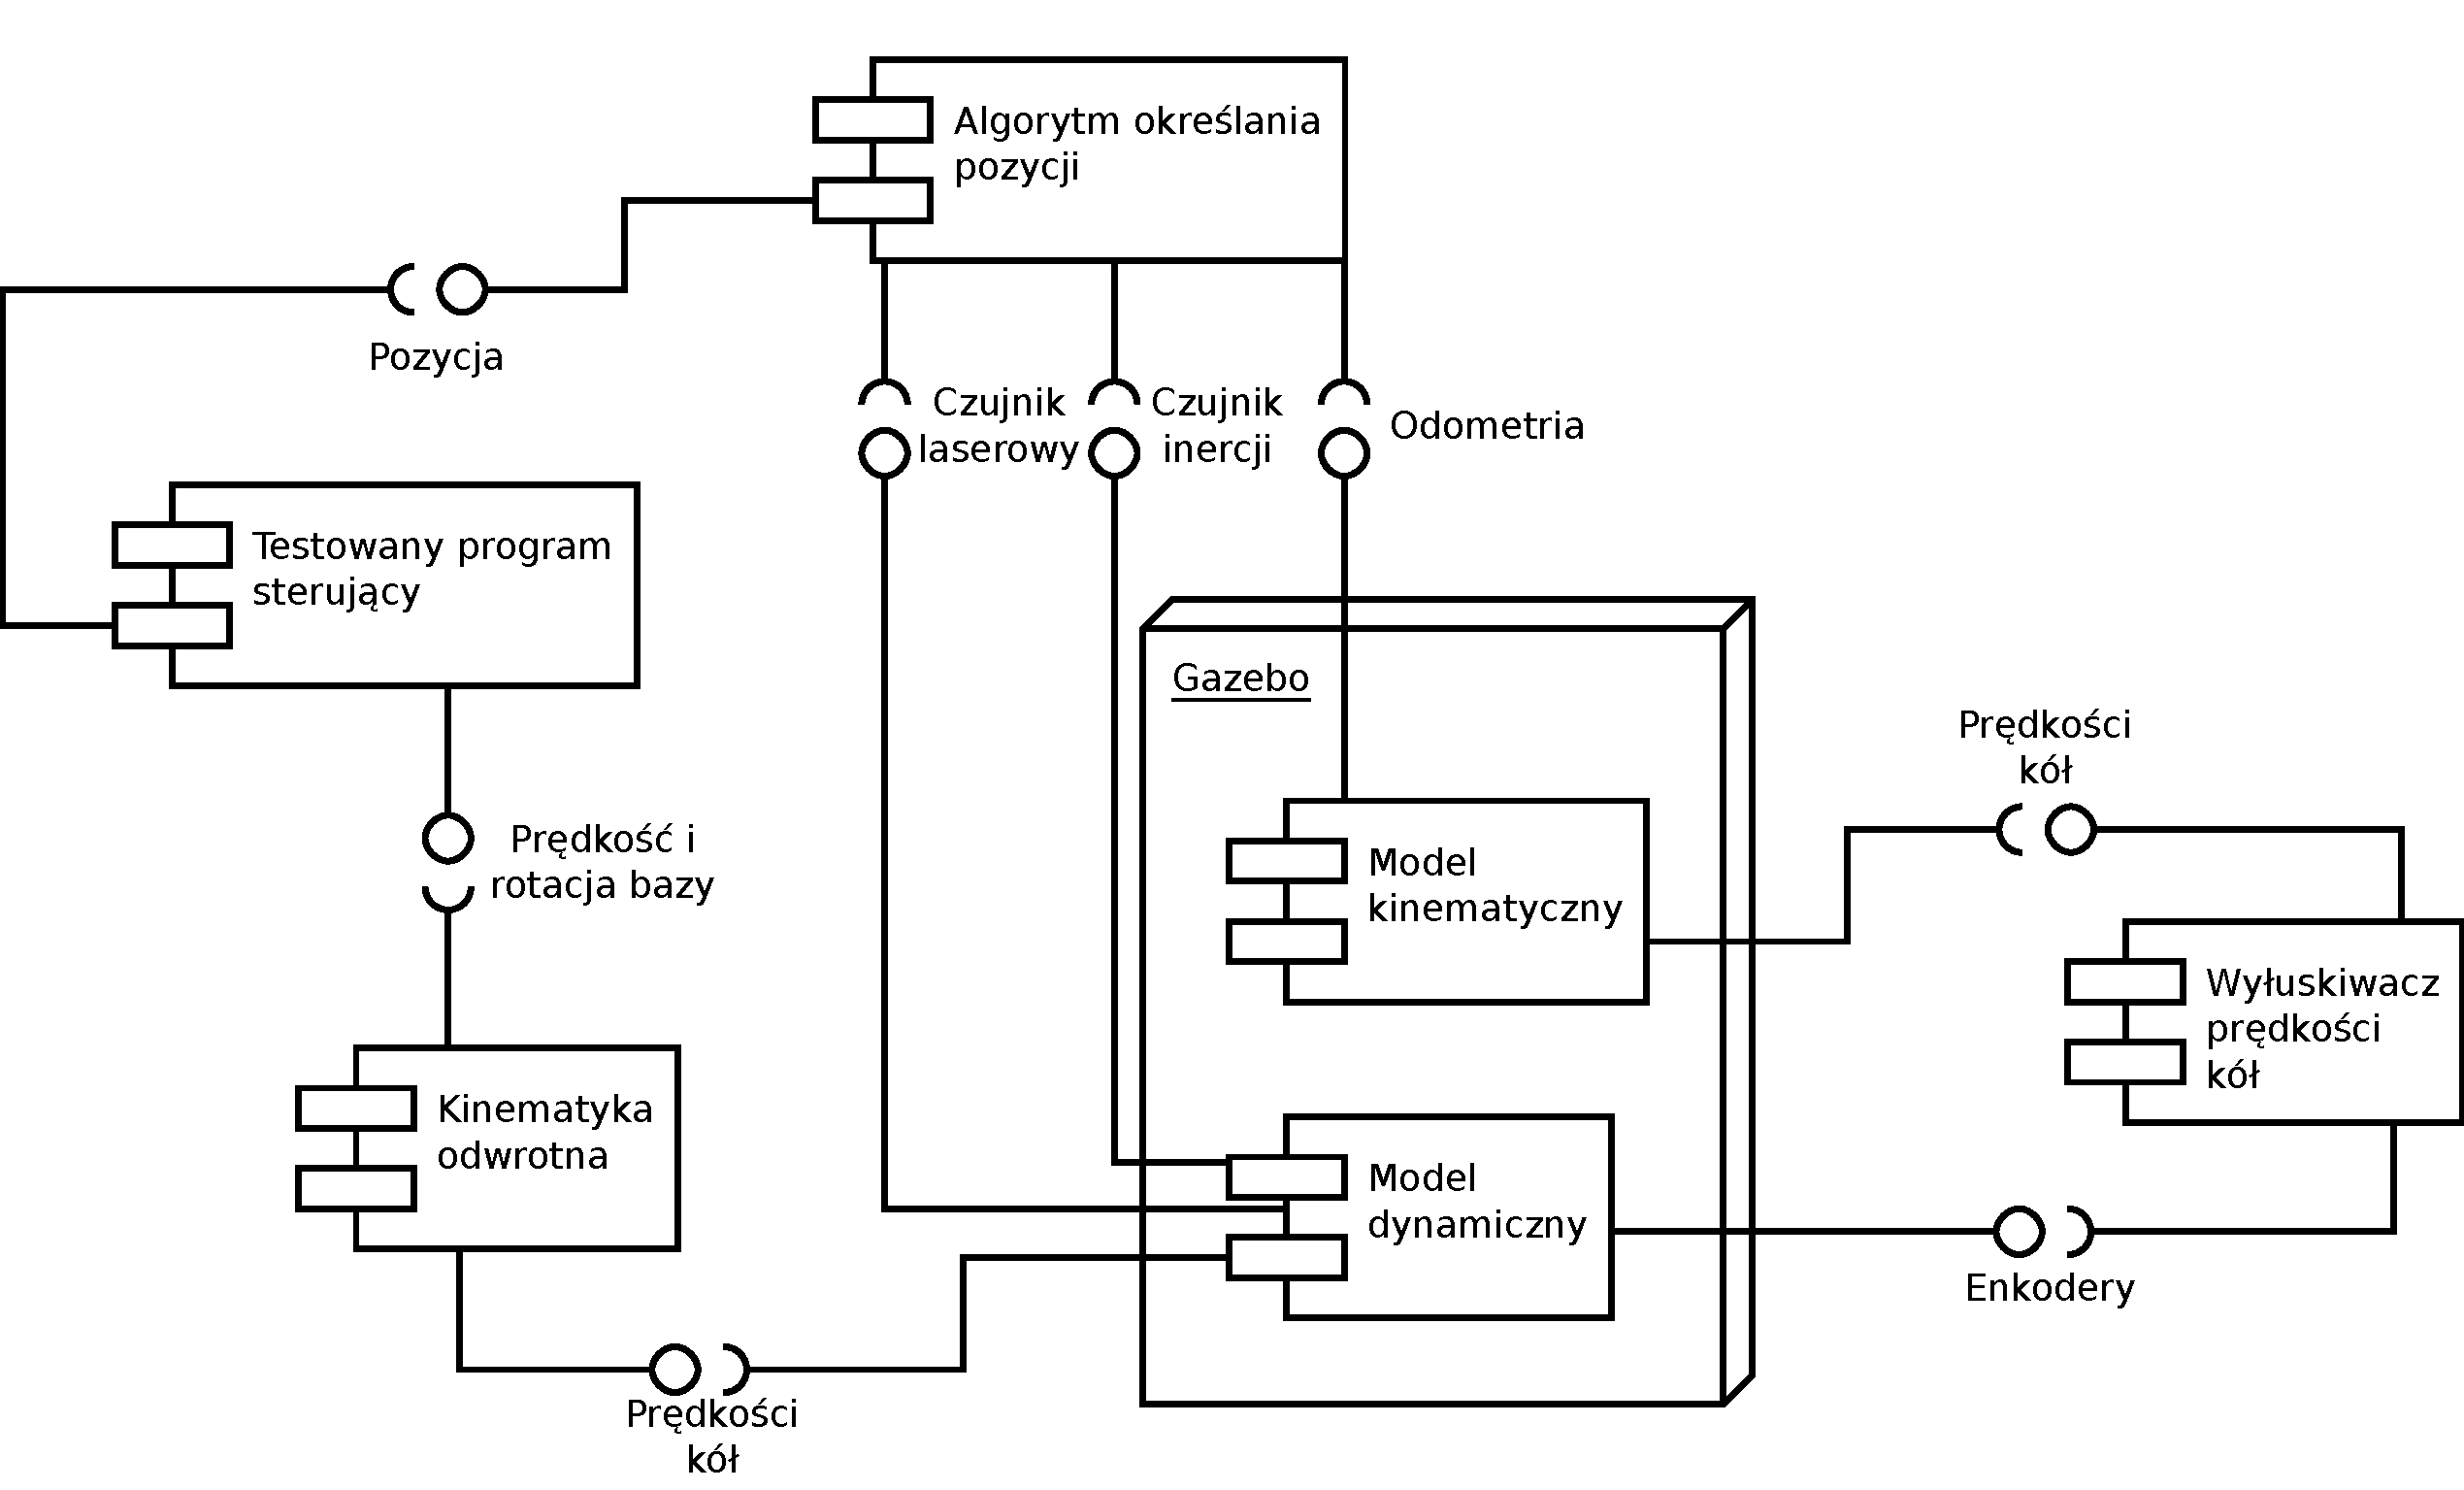
\includegraphics[width=\textwidth]{uml/final.pdf}
	\caption{Komunikacja podstawowych komponentów systemu w trakcie testowania programu sterującego.}
\end{figure} 

Ważną rolę odgrywa tutaj algorytm określania pozycji, bazujący na odometrii, czujniku inercji i danych z czujnika laserowego.
Odometria jest generowana za pomocą modelu kinematycznego, sterowanego danymi z enkoderów modelu dynamicznego.
Sam model dynamiczny sterowany jest pośrednio przez program, który generuje zadane prędkości i obrót robota.
W uproszczeniu: program sterujący wysyła sterowanie do modelu, bazując na jego pozycji, określonej z danych generowanych przez modele czujników.

W każdym miejscu przepływu danych można zebrać i zwizualizować przesyłane wartości.
Program sterujący może także korzystać z czujników laserowych w celu wykrycia przeszkody, nie tylko w celu określenia pozycji.
Bardziej zaawansowany program sterujący mógłby generować zadane prędkości kół bezpośrednio.

Komponenty modeli platform i czujnika laserowego, zostały opisane szczegółowo w poprzednich sekcjach.

\begin{description}
	\item[\texttt{omnivelma}] Model platformy dynamicznej w sekcji \ref{sec:omnivelma}.
	\item[\texttt{pseudovelma}] Model platformy kinematycznej w sekcji \ref{sec:pseudovelma}.
	\item[\texttt{monokl}] Model czujnika laserowego w sekcji \ref{sec:monokl}.
\end{description}


\section{Składniki systemu}
	Środowisko symulacyjne składa się z kilku odrębnych modułów, które komunikują się ze sobą poprzez specjalne interfejsy, wykorzystujące kolejki wiadomości.
	Taka implementacja komunikacji pozwala zmieniać i reimplementować poszczególne elementy i używać różnych języków programowania, 
	zachowując jednolitą komunikację między składnikami i nie tracąc na kompatybilności między komponentami.
	Możliwe jest także przesyłanie wiadomości przez sieć, co pozwala na rozproszenie systemu.

	%TODO Zmienić na Tikz
	\begin{figure}[H]
	\centering
	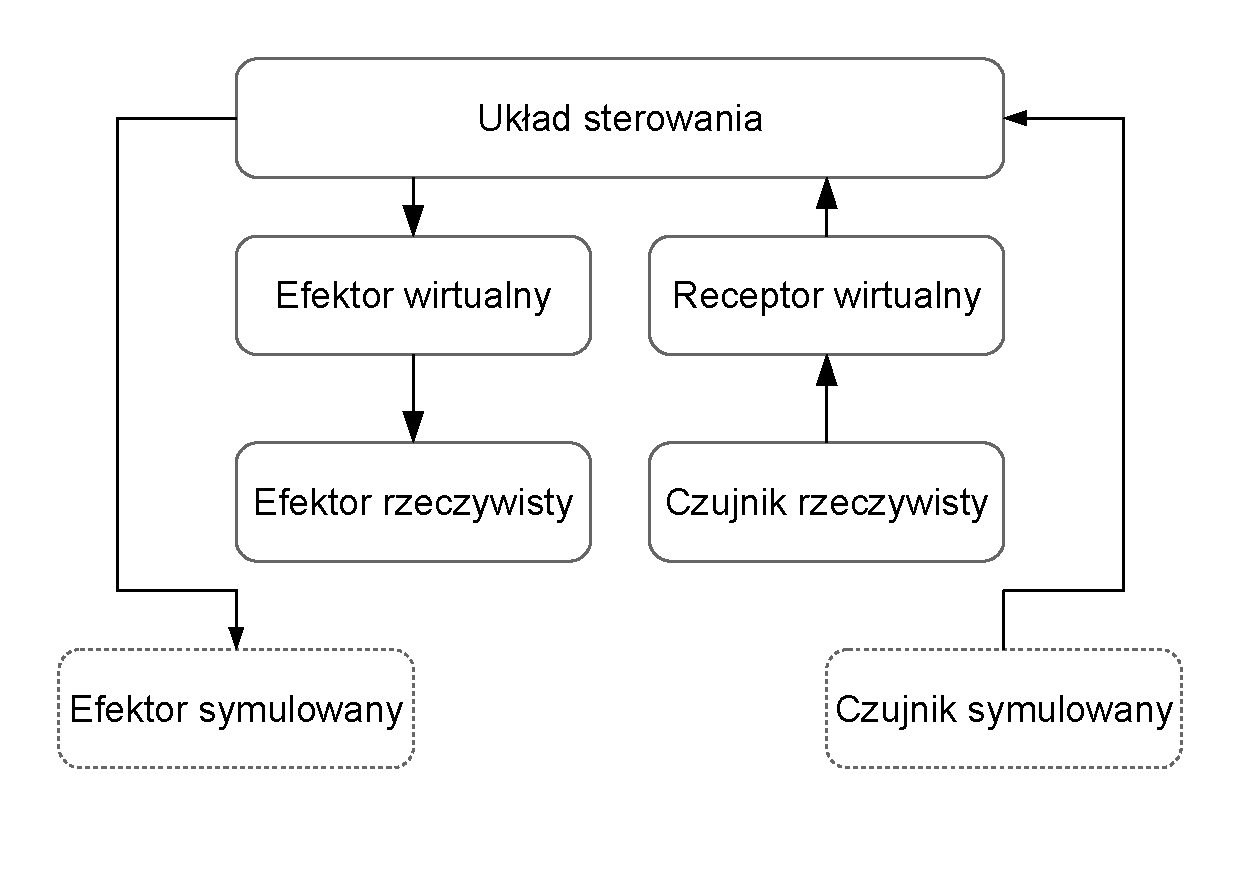
\includegraphics[width=0.8\textwidth]{graphics/agent.pdf}
	\caption{Struktura agenta upostaciowionego.}
	\label{fig:agent}
	\end{figure} 

	Można to przedstawić za pomocą zapisu agentowego, rysunek \ref{fig:agent}.
	Agent upostaciowiony składa się z kilku modułów, komunikujących się ze sobą za pomocą różnych interfejsów.

	Nadrzędnym modułem jest układ sterowania, który na podstawie odczytów z czujników generuje sterowanie dla efektorów.
	Ważne jest, aby komunikacja z rzeczywistymi urządzeniami była identyczna, jak z ich modelami, dzięki czemu taki system będzie przenośny i niezależny od implementacji modelu.

	Efektor rzeczywisty, na przykład serwomotor, jest sterowany za pomocą efektora wirtualnego, który zamienia wyjście układu sterowania na sygnały sterujące dla silnika napędowego.
	Przykładowo, zmienia odebraną liczbę, oznaczającą zadaną prędkość, na odpowiednie napięcie na wyjściu układu sterującego.

	Zamodelowany efektor symulowany również przyjmuje te same sygnały do układu sterowania, co efektor rzeczywisty, 
	lecz nie zamienia ich na sygnały sterujące, a wywołuje odpowiednie funkcje maszyny symulacyjnej, nadające siły i prędkości obiektom w przestrzeni wirtualnej.

	Receptor wirtualny pobiera surowe dane z czujnika, przekształca na odpowiedni format, usuwa błędy i szum tak, aby program sterujący mógł wykorzystać te dane w prosty sposób. 
	Doskonałym przykładem jest tutaj urządzenie Kinect (widoczne na robocie Velma na fotografii \ref{fig:velma}), w którym to zachodzi odczytanie obrazu z kilku kamer.
	Następnie obraz przesyłany jest do komputera, w którym sterowniki interpretują dane, usuwając błędy, tworzą mapę głębokości, wykrywają szkielety i sylwetki osób.
	Te dane mogą być wykorzystane łatwo w grach i programach sterujących.

	Modelowanie receptora, tak jak w przypadku efektora, polega na wygenerowaniu odpowiednich danych, używając odpowiednich funkcji w przestrzeni wirtualnej.
	Mogą one polegać na emitowaniu półprostych, symulujących laser, lub wręcz renderowaniu obiektów, aby uzyskać obraz z wirtualnej kamery.
	Receptor symulowany ma pełną wiedzę o symulowanym świecie, dokładne pozycje i prędkości wszystkich obiektów, dane o kolizjach itp. 
	Pozwala to na łatwe symulowanie receptorów nie mogących mieć odwzorowania w rzeczywistości, co przydatne jest w pierwszych stadiach testowania i wyznaczaniu statystyk.
	Takim przykładem jest model czujnika dokładnej pozycji, rotacji i prędkości w kartezjańskim układzie współrzędnych. 
	Czujniki typu GPS, lub żyroskopy nie generują tak dokładnych pomiarów.

	\subsection{Model 3D}
		Model 3D bazy mobilnej, opisany równaniami matematycznymi, powinien mieć zachowanie zbliżone do oryginału, najbardziej jak to tylko możliwe.
		Musi uwzględniać masy i momenty bezwładności elementów składowych, a także wszystkie tarcia.
		Model obejmuje więzy na ruchome elementy, takie jak koła i rolki, aby umożliwić symulację przegubów.

		Model składa się z elementów, odwzorowujących rzeczywiste części składowe bazy mobilnej.
		Elementy posiadają takie cechy, jak:
		\begin{itemize}
			\item Pozycja w modelu.
			\item Masa.
			\item Moment bezwładności.
			\item Kształt fizyczny.
			\item Materiał fizyczny.
			\item Wygląd.
		\end{itemize}

		Dodatkowo, należy uwzględnić wszystkie więzy, w postaci symulowanych przegubów.
		W przypadku tej bazy istnieje typ więzów o jednym stopniu swobody (zawias), używany przy połączeniu przedniej i tylnej części platformy, oraz 
		jako piasty kół i rolek. Można także uznać, że więzy bez stopni swobody używane są do trwałego połączenia czujników z platformą i transportowanym robotem.
		Więzy mogą oddziaływać siłą na elementy do których są podłączone, symulując silniki.

		Elementy składowe i symulowane przeguby oddziałują bezpośrednio z maszyną do symulacji fizycznej. 
		To kształt, masy i momenty bezwładności brył są argumentami funkcji liczących.
		Maszyna symulacyjna oblicza odpowiednie prędkości i nadaje je podanym obiektom w podobny sposób, jak ma to miejsce w rzeczywistości.

		Do modelu doczepia się wirtualne czujniki, generujące odpowiednie dane na podstawie symulacji i rozkładu losowego.
		Nie są to pełne dane o stanie modelu, jakie posiada maszyna do symulacji, gdyż czujniki fizyczne również nigdy nie mają pełnej informacji o stanie urządzenia.
		Należy dodać losowy szum i błędy, aby przybliżyć ich zachowanie do rzeczywistych czujników.

		Dla ozdoby, można wykorzystać istniejący model CAD do stworzenia siatki trójwymiarowej i nadania symulowanemu obiektowi wyglądu zbliżonego do fizycznego robota.

	\subsection{Sterownik silników}
		Program sterujący generuje abstrakcyjne dane, na przykład liczbę zmiennoprzecinkową, zapisaną binarnie.
		Przykładowy silnik fizyczny nie jest w stanie działać na podstawie takich danych, do pracy potrzebuje odpowiedniego napięcia na wejściu,
		ale interfejs serwomotoru na przykład przyjmuje bardziej abstrakcyjne dane w formie liczby stałoprzecinkowej, jako pole w odebranej ramce.
		Do tłumaczenia jednych danych na drugie, potrzebny jest sterownik niskopoziomowy.
		Najczęściej implementowany jest w formie mikrokontrolera, lub podobnego systemu wbudowanego.

		Jego zadanie to odczytanie danych, podanych przez program sterujący i na przykład generowanie na ich podstawie odpowiedniego przebiegu PWM, lub obsługa przetwornika cyfrowo-analogowego.
		Do innych zadań może należeć kontrola, czy żądana wartość nie uszkodzi urządzenia.
		Zazwyczaj sterownik może komunikować się z powrotem z resztą systemu, aby zgłaszać ewentualne awarie.

		Taki program i powiązany z nim układ elektroniczny są najczęściej dostarczone przez producenta robota i nieznane użytkownikowi.
		Dodatkowo, tworzy to kolejną warstwę abstrakcyjną dla sterownika głównego, który nie musi zważać na generowanie różnych danych dla różnych modeli tych samych efektorów.
		
		W środowisku wirtualnym należy stworzyć moduł o podobnym działaniu.
		Powinien przyjmować dane w dokładnie takim samym formacie, jak opisany wyżej układ, aby był łatwo wymienialny na sterownik fizycznego urządzenia bez ingerencji w główny program sterujący.
		Zamiast zamieniać odczytane dane na analogowe wartości, on wywołuje odpowiednie funkcje maszyny symulacyjnej, aby wywołać taki sam efekt, co na rzeczywistym efektorze, lecz w wirtualnej przestrzeni symulacji.
		Jako argumenty podaje parametry fizyczne symulowanego obiektu, oraz przyłożone siły.
		

	\subsection{Sterownik czujników}
		Implementowany podobnie do sterownika silników, ma za zadanie konwertować surowe i obarczone błędami dane z czujników, na format zrozumiały dla programu sterującego.
		W tym miejscu usuwa się błędy grube, niweluje stałe na podstawie kalibracji, wygładza szum i interpretuje dane, aby pozyskać wymagane przez wyższe warstwy informacje.

		Przykładowo, czujniki laserowe zwracają jedynie ciąg pomiarów, ale to do tego programu należy interpretacja wykrytych kształtów, łączenie punktów i obróbka do formatu zrozumiałego dla wyższych podzespołów.
		Większość zaawansowanych receptorów posiada owe układy cyfrowe i programy wbudowane w urządzenie.
		Dostarczone są przez producenta tak samo, jak sterowniki efektorów.
		
		Aby zasymulować ten element, należy zbudować program generujący dane na podstawie aktualnego stanu maszyny do symulacji, w sposób w jaki działa czujnik w rzeczywistości.
		Na przykład, dla czujnika laserowego, silnik symulacji fizycznej emituje odpowiednią ilość promieni i oblicza ich punkty przecięcia się z wirtualnymi modelami.
		Renderowanie obrazu pozwala na symulację kamery.

		Ponieważ dane fizyczne nigdy nie są idealne, w celu przybliżenia wyjścia wirtualnego czujnika do oryginału, dodaje się szum o odpowiednim rozkładzie i błędy.

	\subsection{Program sterujący}
		W programie sterującym obliczane jest sterowanie, na podstawie dostarczonych odczytów z czujników.
		Zazwyczaj wykorzystuje się tutaj także zewnętrzne biblioteki, dostarczające zaawansowane algorytmy.
		Ich zadania mogą polegać na budowie wewnętrznej mapy, wyznaczaniu ścieżki, omijaniu przeszkód, odwrotnej kinematyce i tym podobnych.

		Taki program zwykle działa na mocniejszych układach logicznych, niż sterowniki, ze względu na duże zapotrzebowania na moc obliczeniową
		i niedeterministyczny czas obliczeń.
		Jeśli robot komunikuje się z użytkownikiem, to zachodzi to w tym module. 

		Programy sterujące mogą być implementowane w językach wysokopoziomowych, nawet skryptowych, gdyż wymagania czasowe nie są rygorystyczne.
		Co więcej, często się zdarza, że odpowiednie składowe programu bazują na różnych technologiach.

		Środowisko symulacyjne powinno zapewnić pełną abstrakcję komunikacji tego modułu.
		Oznacza to, że niezależnie, czy program steruje rzeczywistym robotem, czy symulacją wirtualną, zawsze powinien móc komunikować się i otrzymywać dane w tym samym formacie.
		W idealnym przypadku program nie powinien mieć możliwości stwierdzić, czy steruje symulacją, czy fizycznym urządzeniem.
		

Pierwszym krokiem do stworzenia modelu dynamicznego jest stworzenie modelu kinematycznego, aby móc porównać z nim tworzony model dynamiczny, oraz fizyczną platformę,
w celu weryfikacji poprawności działania.
Dzięki temu, można łatwo oszacować, jak bardzo błędy symulacji, oraz błędy niedoskonałości fizycznego modelu odstają od matematycznych wyliczeń.

Dodatkowo, stworzenie modelu platformy kinematycznej pozwala na proste odrzucanie niedziałających implementacji modelu dynamicznego.
Model platformy kinematycznej ma także kluczowe zastosowanie w odometrii.

\begin{figure}[H]
\centering
 \includegraphics[width=0.8\textwidth]{graphics/base_dims.pdf}
\caption{Wielkości używane we wzorach.}
\label{fig:base_dims}
\end{figure} 

\begin{table}
\centering
\begin{tabular}{c c l}
Oznaczenie & Wartość & Opis \\
\hline
$r$ & 0,1 m & Promień koła w najszerszym miejscu na środku. \\
$a$ & 0,76 m & Szerokość platformy między środkami kół tej samej osi. \\
$b$ & 0,72 m & Długość platformy między środkami kół tego samego boku. \\
$\omega_i$ & & Prędkość kątowa każdego z kół. \\
$v_x$ & & Prędkość transwersalna w osi X. \\
$v_y$ & & Prędkość transwersalna w osi Y. \\
$\omega_z$ & & Prędkość kątowa w osi Z, wektor skierowany w górę. \\
\end{tabular}
\caption{Opisy i wartości symboli używanych we wzorach i rysunkach.}
\label{tab:dims}
\end{table}

\section{Sposób zapisu w formacie SDF}
\label{sec:sdf}
	\emph{Simulation Description Format} (SDF) jest formatem XML, pozwalającym na określenie elementów i zależności pomiędzy nimi w przestrzeni trójwymiarowej, 
	w szczególności budowy i rozmieszczenia robotów.
	Powstał jako zamiennik poprzedniego formatu URDF ze względu na jego skomplikowaną semantykę i brak możliwości określania środowiska wokół robotów, 
	na przykład rozmieszczenie elementów na symulowanej scenie, określania wyglądu i fizycznego zachowania się materiałów itp.

	W przeciwieństwie do poprzednika, zapisującego model w przestrzeni drzewiastej, SDF równolegle określa wszystkie składowe modelu, 
	oraz zależności między nimi jak więzy i względne pozycje.
	Model składowych robota ma strukturę gwiazdową. Jeden element, \texttt{model}, jest nadrzędny, wszystkie składowe są logicznie rozmieszczone równolegle jako podelementy.
	Specjalnie opisane więzy definiują interakcje pomiędzy składowymi.
	Jako model, standard rozumie nie tylko roboty, ale także obiekty typu przeszkody, źródła światła, elementy animowane i tym podobne.
	Standard jest dobrze opisany na stronie internetowej \cite{sdf_website}.

	Element typu \texttt{world}, równoległy do modeli, zawiera informacje o środowisku symulacji.
	Dodatkowo można dodać informację o ustawieniach maszyny symulującej fizykę, wyglądzie sceny, wietrze, grawitacji, polu magnetycznym itp.

	W każdym z modeli zawiera się nazwa, domyślna pozycja, sposób traktowania przez symulator i wtyczki programów obsługujących zaawansowane zachowanie modelu,
	opisane w równoległych do składowych elementach, ale jako że wszystkie te mogą wystąpić tylko raz, należy traktować je jako część elementu \texttt{model}.
	Model, lub jego fragment, może być zaimportowany z innego pliku, lecz nie zmieni to struktury gwiazdowej, a co za tym idzie, może dojść do utraty informacji.
	Ten przypadek zachodzi przy modelach czujników laserowych, opisanych w rozdziale \ref{sec:monokl}.

	Model zawiera w sobie równolegle wszystkie elementy typu \texttt{link}, każdy z nich jest osobną, kompletną częścią robota, na przykład kołem, 
	fragmentem ramienia chwytaka, kadłubem, czujnikiem.
	Składuje w sobie informacje o pozycji względem lokalnego środka układu współrzędnych modelu, masie, kształcie, fizycznym kształcie, materiale fizycznym i wyglądzie.
	Pozwala na dodanie elementów reprezentujących źródła dźwięku, czujniki, baterie itp.

	Same elementy zawierają jedynie informacje o swoim początkowym umiejscowieniu w modelu, ale nie o sposobie poruszania się i nałożonych więzach.
	Do tego potrzebne są, równoległe do elementów \texttt{link}, typy \texttt{joint} określające typ więzów, osie, współczynniki sprężystości, wytrzymałość, czy moc silników.
	Każde połączenie określa, między jakimi obiektami się łączy.
	
	\begin{figure}[H]
	\dirtree{%
	.1 sdf.
	.2 world\DTcomment{Opis przestrzeni symulacji}.
	.2 model\DTcomment{Model w przestrzeni}.
	.3 plugin\DTcomment{Program sterujący modelem}.
	.3 link\DTcomment{Składowa modelu}.
	.4 collision\DTcomment{Fizyczny kształt składowej}.
	.4 visual\DTcomment{Siatka definiująca wygląd składowej}.
	.4 sensor\DTcomment{Czujnik w składowej}.
	.5 plugin\DTcomment{Program sterujący czujnikiem}.
	.3 joint\DTcomment{Wiąz pomiędzy składowymi}.
	}
	\caption{Najważniejsze elementy formatu SDF.}
	\label{fig:sdf_dir}
	\end{figure} 
	
\section{Model kinematyczny}
	\label{sec:pseudovelma}
	Kinematyka to nauka o ruchach obiektów na podstawie nadanych wektorów prędkości.
	Pomija ona takie aspekty jak masa, moment bezwładności, czy siły.
	
	Model kinematyczny jest sterowany funkcjami matematycznymi, 
	zamieniającymi prędkość kątową kół platformy na prędkości transwersalne geometrycznego środka platformy w układzie współrzędnych lokalnych, oraz jego prędkość kątową. 
	Symulator pozwala również na całkowanie tego ruchu, aby uzyskać aktualną pozycję platformy.
	
	Funkcje tłumaczące prędkości kół najwygodniej zapisać w postaci macierzowej, podobnie do tego, jak opisano w \cite{wheels}. 
	Wzór powtarza się w wielu innych pracach naukowych, a jego dokładny kształt zależy od kolejności numerowania kół i interpretacji wymiarów.
	Dla opisanego tutaj przypadku, (stałe zdefiniowane są w tabeli \ref{tab:dims}, numerowanie kół na rysunku \ref{fig:base_dims}):
	
	\begin{equation}
	\begin{bmatrix}
	v_x \\
	v_y \\
	\omega_z \\
	\end{bmatrix}
	=
	\frac{r}{4}
	\begin{bmatrix}
	-1 & 1 & -1 & 1 \\
	1 & 1 & 1 & 1 \\
	\frac{2}{a+b} & \frac{-2}{a+b} & \frac{-2}{a+b} & \frac{2}{a+b} \\
	\end{bmatrix}
	\begin{bmatrix}
	\omega_1 \\
	\omega_2 \\
	\omega_3 \\
	\omega_4 \\
	\end{bmatrix}
	\end{equation}
	
	Uzyskane wartości należy przemnożyć przez odpowiednie wektory jednostkowe, obrócić względem lokalnego układu współrzędnych dla modelu i zastosować w funkcjach nadających prędkości bryle.

	Ponieważ sterowanie pozycją modelu kinematycznego odbywa się wyłącznie poprzez wzory matematyczne, w jego symulacji nie uczestniczy maszyna symulacyjna fizyki.
	Taki model nie reaguje na kolizje z innymi obiektami, nie reaguje na różnicę terenu i nie używa informacji o współczynnikach tarcia materiałów, tak jak model dynamiczny.

	Nazwa kodowa \texttt{pseudovelma} odnosi się do tego, że jest to nieprawdziwy ruch sterowany z zewnątrz, a nie prawdziwa symulacja.

	\subsection{Problemy implementacji}
		Gazebo nie ma zaimplementowanego pełnego wsparcia dla standardu SDF.
		W szczególności nie działa struktura elementów \texttt{frame}, odpowiadająca za transformacje obiektów względem innych obiektów.
		Nie jest to zapisane w dokumentacji, a jedynie zgłoszone od kilku lat w systemie kontroli wersji jako błędy.

		Oznacza to, że wszystkie elementy typu \texttt{link}, będąc dziećmi \texttt{model}, nie zachowują swojej pozycji w lokalnym układzie współrzędnych.
		Powoduje to, że nadając prędkość kątową modelowi za pomocą funkcji, nadajemy ją każdej składowej osobno.
		Każde z kół i dwie części bazy, obracają się zgodnie z zadanymi wartościami, ale ich środki pozostają w miejscu, w którym rozpoczęły symulację,
		ignorując kompletnie pozycję zdefiniowaną dla elementu rodzica \texttt{model}.
		
		Z punktu widzenia symulacji fizycznej ma to sens, gdyż nie można zakładać że składowe modelu są w jakikolwiek sposób podłączone do jego głównej części
		(która wcale nie musi mieć zdefiniowanego kształtu fizycznego), to wprowadzałoby także nieścisłości w typie połączenia, niektóre elementy powinny być przecież ruchome.

		Aby przeciwdziałać temu zjawisku, należy przenieść zawartość elementów \texttt{link} do elementu \texttt{model} i ustawić je jako \texttt{visual} elementu \texttt{model}.
		W ten sposób traktowane są jako część renderowana modelu, a nie osobne składowe.
		Nie można użyć tutaj więzów statycznych, gdyż te są wykorzystywane przez maszynę symulacyjną fizyki i ignorowane są przy kinematycznym ruchu.

		Powstała niedogodność jest taka, że ciężej jest sterować obrotem elementów \texttt{visual}, gdyż są zarządzane przez kompletnie inny system symulatora,
		służący do graficznego renderowania sceny.
		Oczywiście ma to znaczenie jedynie kosmetyczne, gdyż w żaden sposób nie wpływa na ruch modelu bazy.

	\subsection{Komunikacja}
		Komunikacja programu sterującego platformą odbywa się przez wbudowane z ROSa narzędzie \emph{topic}.

		Wiadomość zawierająca dane prędkości kół czterokołowego robota nie mieści się w standardzie, zatem został stworzony specjalny typ \texttt{omnivelma\_msgs/Vels}.
		Ta stryktura zawiera cztery wartości zmiennoprzecinkowe podwójnej precyzji, oznaczające prędkości w $\frac{rad}{s}$.

		Program w każdym cyklu symulacji nadaje wiadomości:
		\begin{itemize}
		\item \texttt{geometry\_msgs/PoseStamped} z aktualną pozycją i rotacją platformy, oraz nagłówkiem z identyfikatorem i czasem nadania pakietu.
		\item \texttt{geometry\_msgs/TwistStamped} z aktualną prędkością platformy, oraz identycznym nagłówkiem.
		\item \texttt{nav\_msgs/Odometry} z obiema powyższymi danymi i nagłówkiem. Służy przy obliczaniu ruchów platformy na podstawie enkoderów kół.
		\end{itemize}
		Ponadto program przyjmuje dane:
		\begin{itemize}
		\item \texttt{omnivelma\_msgs/Vels} z zadanymi prędkościami kół.
		\end{itemize}

	\subsection{Zachowanie}
		Platforma ignoruje kompletnie otoczenie, poruszając się przez inne obiekty na scenie.
		Po nadaniu stałych prędkości kół, następuje ruch po okręgach zgodnie z rysunkiem \ref{fig:mecanum_dirs}.

		Program sterujący, co każdą klatkę symulacji (okres zależy od zasobów procesorowych komputera), zwraca aktualną pozycję i rotację, 
		działając jak układ całkujący funkcje ruchu z powyższej macierzy.

\section{Model dynamiczny}
	\label{sec:omnivelma}
	Wykorzystując maszynę do symulacji fizyki, można umieścić w niej model określający kształty, masy i zależności pomiędzy składowymi modelu, 
	następnie nadać elementom wirtualne siły i otrzymać przybliżone wyniki do tego, jak zachowywałaby się rzeczywista platforma.

	Wszystkie programy i definicje związane z tym modelem noszą nazwę \texttt{omnivelma}, co nawiązuje do wielokierunkowości ruchów robota manipulującego, którego podstawa ma transportować.

	Robot jest bryłą, na którą składają się następujące części składowe:
	\begin{itemize}
	\item Główna część trzonu.
	\item Ruchoma, mniejsza część trzonu, z przodu robota.
	\item 4 koła, 2 podłączone do głównej części, a 2 do przedniej.
	\item Po 12 rolek na każdym kole.
	\item Przegub zawiasowy, łączący dwie części podstawy.
	\item 4 przeguby zawiasowe z silnikami, łączące części bazy z kołami.
	\item 12 przegubów zawiasowych na każdym kole, łączących koła z rolkami.
	\end{itemize}

	Jest to dość skomplikowany obiekt do symulacji, dlatego należy skłonić się do znalezienia sposobu na uproszczenie modelu, w celu zmniejszenia ilości obliczeń symulatora
	i błędów reprezentacji liczb zmiennoprzecinkowych.

	Istnieje wiele podejść do stworzenia odpowiedniego modelu. Każde z nich było proponowane na różnych forach przez osoby symulujące podobne bazy, a także w zawartej bibliografii.
	
	Jednak idealne rozwiązanie nigdy nie zostało znalezione.
	Działający w tym przypadku sposób także nie został wcześniej sprawdzony.

	\subsection{Jak największe zbliżenie do oryginału}
		Wspomniany wyżej sposób jest najbardziej wymagającym obliczeniowo, ale także najprostszym z możliwych.
		Należy stworzyć elementy składowe systemu i nadać im fizyczny kształt za pomocą odpowiedniej siatki trójkątów.
		Kształt obiektów może być także ustalony jednym prymitywów, jak sześcian, kula, łamana, walec i płaszczyzna.
		Takie przybliżenie znacznie przyspiesza obliczenia, gdyż może być specjalnie traktowane przez algorytmy.

		Słabym punktem tego rozwiązania jest fakt, że rolki są niestandardowym kształtem, opisanym dokładniej w \cite{rollers}, 
		którego dokładność jest bardzo wysoce wymagana dla zmniejszenia niedokładności ruchów.
		Przybliżenie jej walcem powoduje problemy przy przenoszeniu punktu podparcia na kolejną rolkę, gdyż koło będzie musiało przez chwilę oprzeć się o krawędź.
		Taki model samoczynnie drgałby przy obrocie koła, zwiększając tym samym i tak duże niedokładności. 
		Podejście to zostało także zaproponowane w innej pracy naukowej \cite{modelling_ways}.

		Przybliżenie rolki siatką jedynie zmniejsza powyższy efekt, gdyż sama siatka zbudowana jest z prostych odcinków.
		Zwiększając jej gęstość można teoretycznie poprawić jakość symulacji, kosztem olbrzymiego skoku ilości obliczeń, każde obarczone błędami liczbowymi.
		Kalkulowanie kolizji fizycznej siatek jest najdroższe ze wszystkich obliczeń kolizji w maszynach symulacji fizyki.

	\subsection{Resetowanie pozycji koła}
		Ten sposób został użyty w modelach w symulatorze V-Rep.

		Polega on na tym, iż koło, podłączone do bazy, posiada przegub zawiasowy, obrócony pod kątem 45° w stosunku do osi koła, tak aby był równolegle do aktualnie dolnej rolki.
		Do tego przegubu podłączona jest kula reagująca z podłożem, którą to w każdej iteracji symulacji należy zresetować do pozycji wyjściowej, razem z przegubem.
		Kula jest prymitywem i obliczenia jej kolizji są najmniej wymagające obliczeniowo dla maszyny symulacyjnej.

		\begin{figure}[H]
		\dirtree{%
		.1 kadłub\DTcomment{Podstawa bazy}.
		.2 przegub z silnikiem\DTcomment{Nadaje moment obrotowy na żądanie}.
		.3 wirtualne koło\DTcomment{Obiekt bez kształtu, obraca się jak koło}.
		.4 siatka\DTcomment{Odpowiada za wygląd obiektu koła}.
		.4 przegub 45°\DTcomment{Obrócony pod kątem 45°}.
		.5 kula kształtu\DTcomment{Uczestniczy w symulacji fizyki}.
		}
		\caption{Zagnieżdżenie obiektów koła z resetowaną symulacją rolki.}
		\label{fig:vrep_wheel}
		\end{figure}

		Wywołuje to takie działanie, jak gdyby koło w danej chwili mogło obracać się w dwóch kierunkach, tak jak aktualnie najniższa rolka i tak jak wymusza to na kole 
		symulator silnika mechanicznego.
		Przez następną klatkę symulacji, model zachowuje się poprawnie, aż obrót głównej osi zaczyna negatywnie wpływać na symulację,
		zmieniając kąt wewnętrznego przegubu, przez co przestaje być równoległy do dolnej rolki.
		Zanim jednak ten efekt się nasili, jego rotacja jest przywracana do pozycji początkowej.
		Ponieważ jest to wywoływane poprzez zmianę rotacji, a nie nadanie momentu obrotowego obiektowi, 
		maszyna symulacyjna nie bierze w takim przypadku pod uwagę tarcia kuli o podłoże. 

		Niestety, nie jest możliwe uzyskanie tego rozwiązania wprost w Gazebo, gdyż struktura drzewiasta obiektów nie jest zaimplementowana, jak to wcześniej zostało opisane.
		Co więcej, metody natychmiastowo zmieniające pozycje obiektu nie działają poprawnie.
		W dodatku, potrzebna jest także możliwość ustawiania rotacji i pozycji przegubu, elementu \texttt{joint}, co nie jest wystawione do modyfikacji w API.

		Bardzo skomplikowany sposób działania kół skłania do szukania innych rozwiązań.

		Taka budowa koła ma jeszcze jedną, ważną cechę. 
		Jakość symulacji zależy od jej prędkości.
		Jest tak, ponieważ im bardziej obciążony jest symulator, tym większy czas pomiędzy kolejnymi klatkami symulacji i pomiędzy kolejnymi resetowaniami pozycji koła.
		Oznacza to, że druga oś zaczyna wpływać na symulację z nieliniowo rosnącym błędem, aż do kolejnego resetu koła.
		Przy odpowiednio niskim czasie odświeżania, różnice powodują nieakceptowalny spadek jakości symulacji.

	\subsection{Zmiana osi rolki}
		Poprzedni przypadek można zmodyfikować, poprzez wyznaczanie nowej osi przegubu, łączącego wirtualne koło z kulą symulującą rolkę.
		Takie rozwiązanie nie wymaga przywracania rotacji obiektów do poprzedniej wartości, a co za tym idzie, może być użyte w symulatorze Gazebo.

		Oś wewnętrzna podłączona jest do koła wirtualnego i obraca się razem z nim.
		W każdym cyklu należy zamienić, obróconą już w tej klatce oś, na kierunek pierwotny względem postawy platformy.
		Spowoduje to, że kolejna iteracja fizyki będzie mogła obracać kulą reprezentującą rolkę pod odpowiednim kątem.

		Należy obliczyć kierunek osi w przestrzeni globalnej, biorąc pod uwagę aktualną pozycję platformy i obrót kół.
		Obliczenia tego kierunku są złożone.

		Potrzeba jest jeszcze wybrania momentu wyznaczania nowego kierunku osi, bowiem maszyna symulacyjna wywołuje wiele różnych funkcji w jednym cyklu symulacyjnym.
		Zależnie to tego, który moment czasowy się obierze, można spodziewać się różnego zachowania modelu.

		Implementacja tej budowy niestety nie stworzyła działającego rozwiązania.
		Wykonywanie kodu w różnych momentach symulacji nie wpływało na efekt.
		Platforma poprawnie poruszała się jedynie do przodu i do tyłu. 
		Pierwszy problem pojawiał się, gdy w czasie ruchu na bok, prędkość malała, aby zmienić zwrot pomimo niezmiennej prędkości kół.
		Po kilku sekundach problem się powtarzał. Takie zachowanie najczęściej spowodowane jest zachowaniem kierunku osi w lokalnym układzie współrzędnych koła.

		Drugim problemem był ruch po krzywej, w której model nieregularnie podskakiwał, w końcu nawet obracając się w pionie.
		Takie zachowanie oczywiście dalekie jest od oryginału.

		Prawdopodobnie problemem było wewnętrzne traktowanie przegubów przez maszynę symulacyjną.
		Takie nienaturalne zachowanie, jak nagła zmiana osi przegubu, musiała wprowadzać nieprawidłowe wartości do zmiennych stanu, 
		co w rezultacie powodowało tak chaotyczny ruch.

	\subsection{Modyfikacja kierunków i wartości wektorów tarcia}
		\label{sec:friction}
		Warto tu wytłumaczyć, w jaki sposób maszyny symulacji fizyki interpretują kolizję i dotyk.

		\begin{figure}[H]
		\centering
		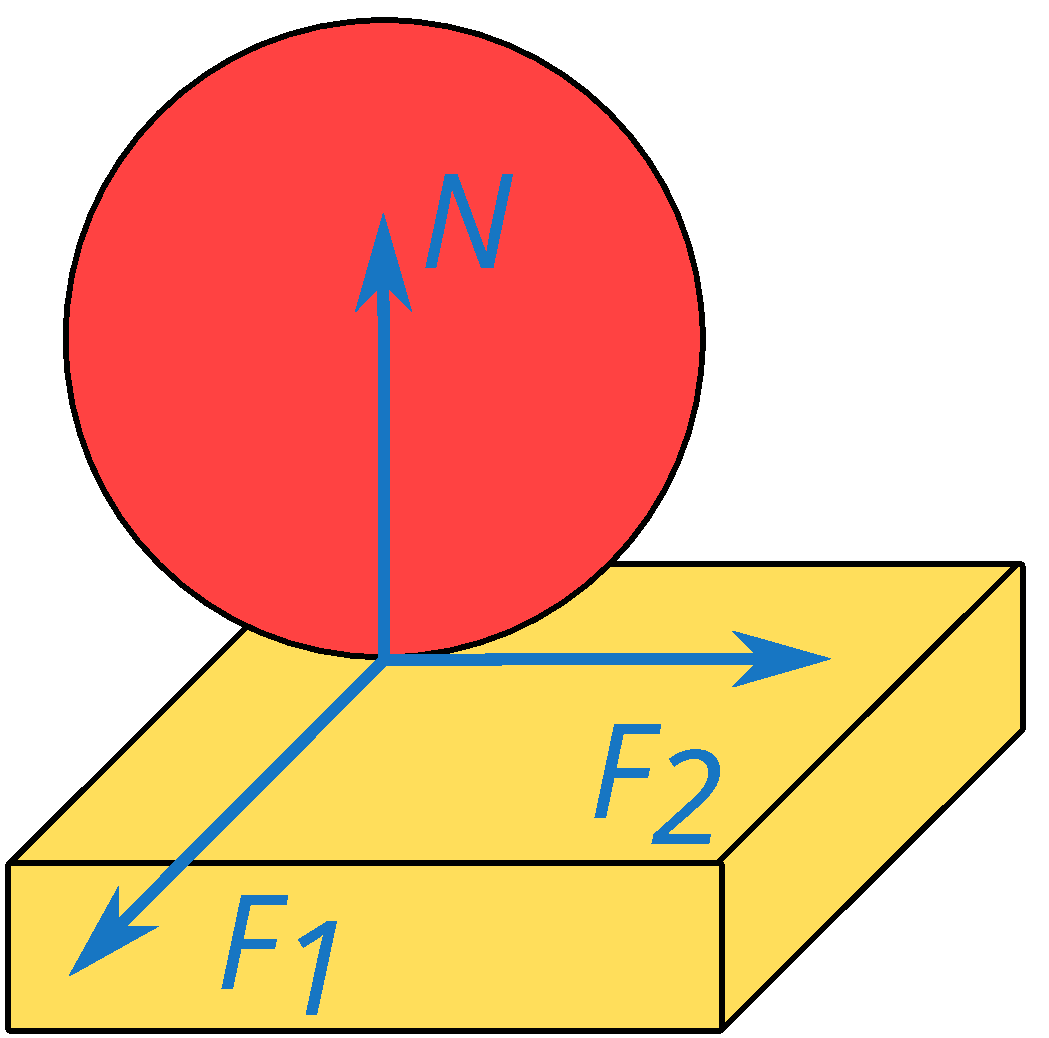
\includegraphics[width=0.5\textwidth]{graphics/friction.pdf}
		\caption{Wektory punktu kolizji.}
		\end{figure} 

		Po wykryciu punktu kolizji i wyznaczeniu wektora normalnych $N$ do dotykających się obiektów, system powinien zadziałać odpowiednimi siłami, 
		aby zatrzymać, lub odbić obiekty od siebie.
		Dodatkowo, ponieważ prędkości obiektów nie muszą być równoległe do wektora kolizji, należy zasymulować siłę tarcia z odpowiednią dla współczynnika tarcia wartością.
		Można to uzyskać, nadając obiektom w punkcie kolizji siłę prostopadłą do wektora normalnych, 
		ten wektor może być rozpisany przy pomocy dwóch wektorów jednostkowych $F_1$ i $F_2$. 
		Te wektory zawsze są prostopadłe do wektora normalnych, równoległe do płaszczyzny kolizji.

		W normalnej symulacji fizyki nigdy nie potrzeba osobno modyfikować współczynników tarcia i kierunku tych wektorów, 
		gdyż zazwyczaj powierzchnie symulowanych obiektów mają równe współczynniki tarcia w każdym kierunku.
		Jednakże modyfikując te wektory statycznie, lub dynamicznie, można uzyskać bardzo interesujące efekty.
		Instrukcja silnika symulacji podaje przykład, w którym aby zamodelować tarcie opon samochodu na zakręcie, prostopadle do kierunku jazdy, 
		należy dynamicznie zmieniać współczynnik tarcia dla wektora $F_1$, lub $F_2$ w kierunku promienia koła.
		Ten współczynnik tarcia, prostopadły do kierunku jazdy, może być liniowo zależny od prędkości.
		Spowoduje to, że im większa prędkość samochodu, tym boczna siła odśrodkowa bardziej wpłynie na tor jego jazdy, co ma odwzorowanie w rzeczywistości.
		Więcej informacji można znaleźć na stronie instrukcji maszyny symulacyjnej ODE \cite{ode_contact}.

		W opisywanym tutaj modelu, modyfikuje się wektor $F_1$, oraz współczynniki tarcia w obu kierunkach, aby przybliżyć zachowanie się rolki.
		Ponieważ wektory $F_1$ i $F_2$ są określone w lokalnym dla koła układzie współrzędnych, 
		w każdej iteracji maszyny symulacji należy obrócić je względem aktualnej pozycji bazy i odwrotności obrotu koła.
		Idealna rolka obraca się całkowicie bez tarcia, a ruch wzdłuż jej osi jest niemożliwy.
		Można więc ustawić zerowy współczynnik tarcia w kierunku prostopadłym do osi, oraz nieskończenie duży dla wektora równoległego do osi.

		\begin{figure}[H]
		\centering
		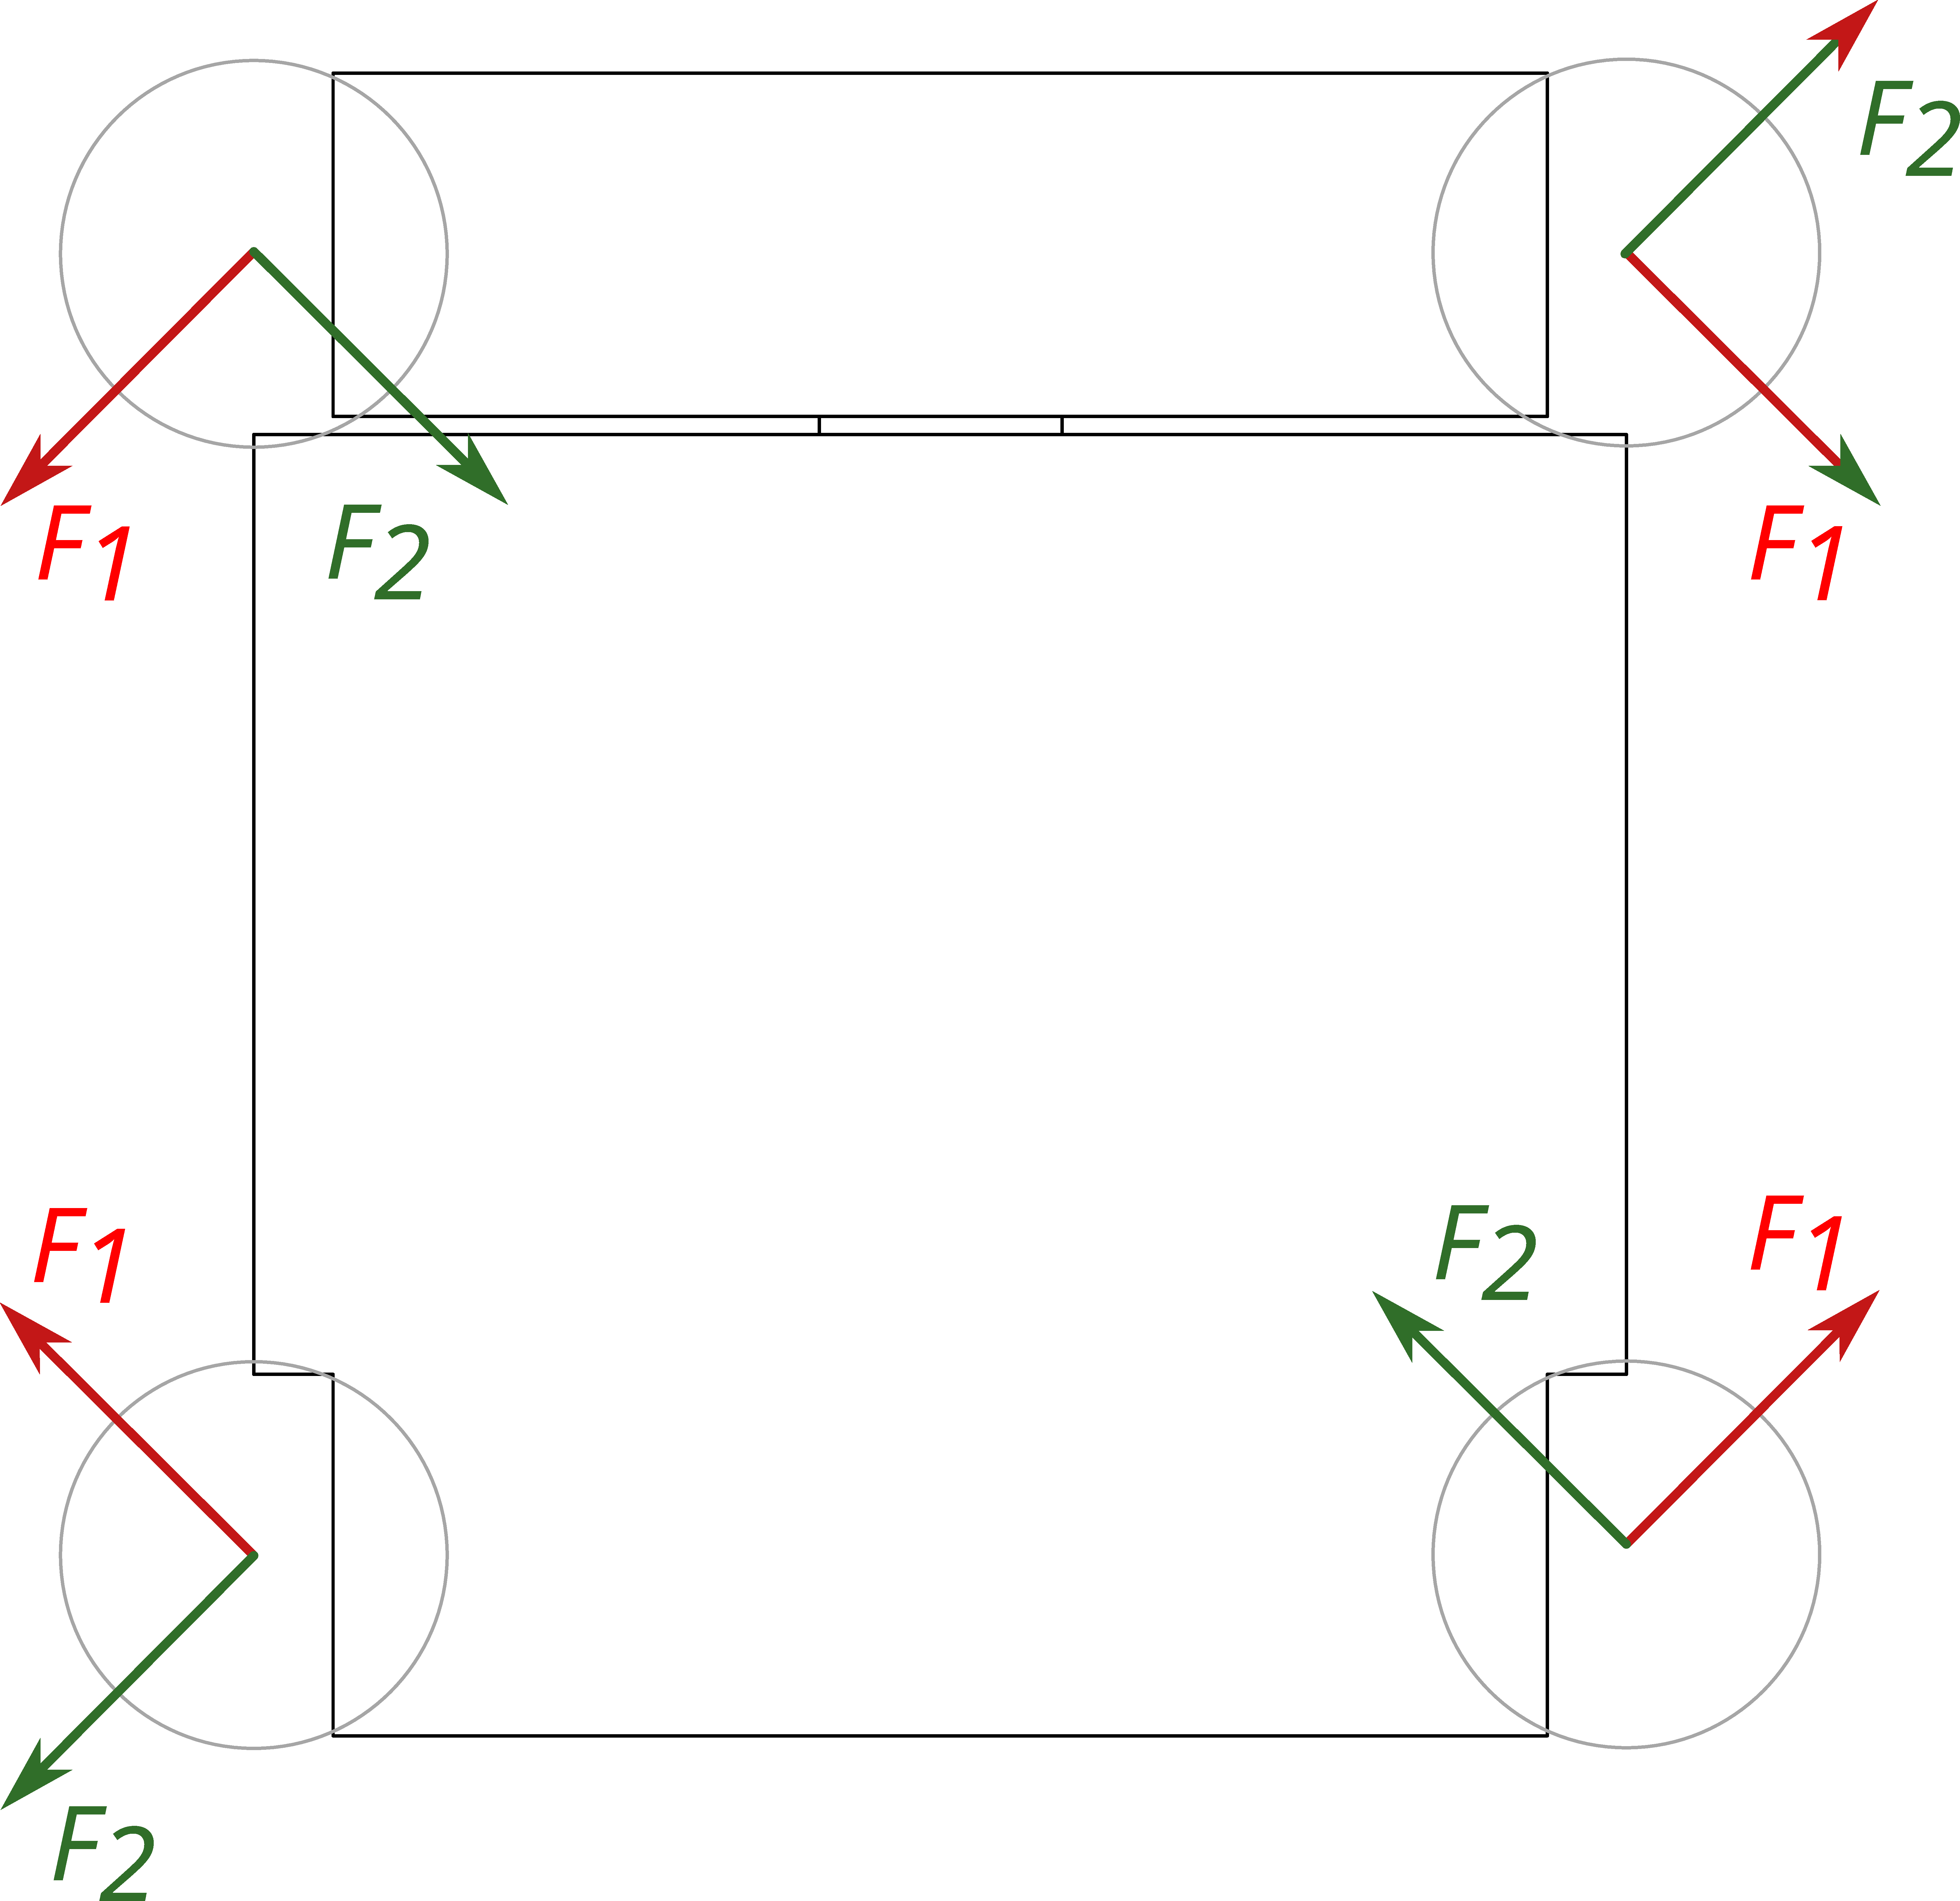
\includegraphics[width=0.8\textwidth]{graphics/base_vects.pdf}
		\caption{Kierunki wektorów dla których należy nadać współczynniki tarcia przy symulacji platformy, widok z góry. Tarcie w kierunku $F_1$ powinno być nieskończone, a w $F_2$ zerowe.}
		\end{figure} 

		Niestety, w rzeczywistości rolki wykonane są ze śliskiego plastiku, który zezwala na poślizg kół wzdłuż ich osi.
		Osie kolek również nie obracają się płynnie, trzeba użyć dużej siły, aby obrócić dowolną z nich, pod naciskiem platformy tarcie jest jeszcze większe.
		Każda rolka obraca się z innym tarciem wprowadzając kolejne zakłócenia.
		Podłoże po którym porusza się robot także nie jest tu bez znaczenia.
		Należy zatem wystawić interfejs do łatwej zmiany współczynników tarcia, aby później dobierać odpowiednie wartości na podstawie zachowania rzeczywistego robota.

		Podobnie, jak w poprzednich przypadkach, modeluje się tylko najniższą, dotykającą podłoża rolkę.
		Jak wcześniej wspomniano, ma ona bardzo skomplikowany kształt, lecz można przybliżyć całe koło kulą.
		Zatem w miejscu każdego koła zamontowana jest kula z dynamicznie modyfikowanym tarciem i siatką w kształcie koła do wizualizacji, 
		oraz przegub z motorem łączący odpowiednią część bazy z kołem.
		To najprostsza budowa modelu (a zatem najszybsza) z poprzednich.
		
		\begin{figure}[H]
		\dirtree{%
		.1 kadłub\DTcomment{Podstawa bazy}.
		.2 przegub z silnikiem\DTcomment{Nadaje moment obrotowy na żądanie}.
		.3 kula\DTcomment{Modyfikowane wektory tarcia}.
		.4 siatka\DTcomment{Odpowiada za wygląd obiektu koła}.
		}
		\caption{Zagnieżdżenie obiektów koła w strukturze drzewiastej z modyfikowanymi wektorami tarcia. W implementacji Gazebo przegub i kula są zagnieżdżone równolegle.}
		\label{fig:omnivelma_wheel}
		\end{figure}

		Takie rozwiązanie wiąże się z pewnym ryzykiem.
		Wymaga, aby symulator używał maszyny ODE, co zmniejsza przenośność modelu. ODE jest domyślnym symulatorem w Gazebo.
		Maszyna Bullet również liczy kolizje w ten sposób i ma modyfikowalne wektory, 
		lecz nie daje podobnych wyników. Być może jest to spowodowane brakiem odpowiedniej konfiguracji, lub innym wewnętrznym traktowaniem modelu.

	\subsection{Komunikacja}
		Ze względu na wiele ustawień elementów bazy, należy stworzyć bogaty interfejs.
		W każdym cyklu symulacji, program sterujący modelem platformy nadaje wiadomości:
		\begin{itemize}
		\item \texttt{geometry\_msgs/PoseStamped} z aktualną pozycją i rotacją platformy, oraz nagłówek z czasem i identyfikatorem.
		\item \texttt{geometry\_msgs/TwistStamped} z aktualną prędkością platformy i nagłówkiem.
		\item \texttt{omnivelma\_msgs/EncodersStamped} z odczytaną ze stanu obiektów kół aktualną rotacją i pozycją, z nagłówkiem. 
		To jest symulator enkoderów wbudowanych w silniki platformy.
		\end{itemize}
		
		Przyjmowane są także dane:
		\begin{itemize}
		\item \texttt{omnivelma\_msgs/Vels} z zadanymi prędkościami kół.
		\item Wywołanie ustawiające współczynniki tarcia wzdłuż wektorów $F_1$ i $F_2$.
		\item Wywołanie ustawiające masy i momenty obrotowe niektórych elementów składowych konstrukcji.
		\end{itemize}

	\subsection{Rozszerzenie modelu}
		\label{sec:model_nan}
		Ponieważ komputerowa reprezentacja liczby zmiennoprzecinkowej pozwala na zapisanie nie tylko liczbowych wartości, można rozszerzyć model o dodatkową funkcjonalność,
		wywoływaną wysłaniem do modelu cichej nie-liczby (\emph{NaN}) w wiadomości, w polu prędkości odpowiedniego koła. 
		Cicha nie-liczba powstaje w procesorze, w module operacji zmiennoprzecinkowych, przy przeprowadzaniu nieprawidłowych, 
		acz niekrytycznych obliczeń, na przykład dzielenie przez zero, lub dzielenie nieskończoności przez minus-nieskończoność 
		(także zapisywane jako forma liczby zmiennoprzecinkowej).
		Takie operacje nie powodują błędu programu, jedynie wynik w postaci nie-liczby propaguje przez wszystkie pozostałe operacje.

		Nadanie prędkości modelom w przestrzeni wirtualnej polega na wywołaniu odpowiedniej funkcji maszyny symulującej fizykę.
		Można zadać pytanie, jak zachowa się model, jeśli dla niektórych kół nie zmieniać prędkości po każdym odebraniu pakietu?

		Wobec tego, jeśli w pakiecie z nowymi prędkościami kół znajdzie się cicha nie-liczba, program sterujący nie nada nowej prędkości temu kołu.
		Jest to podobne do nadania tej samej prędkości, jaką posiada aktualnie obiekt koła (jaką zwróciłby enkoder).

		Zwraca to uwagę również na potrzebę, aby program do komunikacji z rzeczywistym robotem nie skończył się błędem po odebraniu jednej z takich nieokreślonych wiadomości.
		Ponieważ przekształca liczby zmiennoprzecinkowe, zawarte w ROSoswych pakietach, na dane zrozumiałe przez sterownik silnika, które zazwyczaj są liczbami
		stałoprzecinkowymi, program może zachować się nieprzewidywalnie.
		
\section{Model czujnika laserowego}
	\label{sec:monokl}
	Ponieważ czujniki laserowe tego typu są popularnie używane w robotyce, standard SDF posiada dedykowane elementy do umieszczenia takich obiektów w symulacji.
	Również Gazebo posiada możliwość renderowania zasymulowanych impulsów lasera.
	Tak, jak model platformy, ten pakiet otrzymał nazwę kodową \texttt{monokl}, ponieważ pozwala obserwować otoczenie, jak okular.

	\subsection{Obliczenia symulatora}
		Czujnik laserowy jest bardzo łatwo zasymulować w przestrzeni wirtualnej za pomocą rzutowania półprostych.
		Ta technika używana jest w bardzo wielu aspektach komputerowego generowania obrazu i symulacji fizyki.

		Półprosta jest emitowana z ustalonego punktu w pewnym kierunku w przestrzeni trójwymiarowej.
		Następnie system próbuje znaleźć pierwszy punkt jej kolizji z każdym z obiektów o fizycznym kształcie, uczestniczących w symulacji.
		
		Ponieważ zasoby komputera zawsze są ograniczone, długość promienia także musi mieć pewien limit. 
		Zwykle jest on jednak na tyle duży, że z punktu widzenia obiektów uczestniczących w symulacji, w opisywanym tutaj zagadnieniu, 
		można uznać tą odległość za nieskończoną.

		Algorytm obliczania kolizji z półprostą bazuje na kosztowym porównywaniu pozycji każdego obiektu fizycznego na scenie.
		Istnieją oczywiście sposoby na zmniejszenie ilości obliczeń, na przykład metoda prostopadłościanów zawierających obiekt, ale sposób radzenia sobie z tym zagadnieniem nie jest
		częścią tematu pracy,
		Wystarczy wspomnieć, że symulacja dużej ilości laserów oraz obiektów jest operacją kosztowną.
		
		Testy pokazują, że samo ich renderowanie spowalnia symulację około czterokrotnie.
		To ze względu na bardzo dużą ich ilość, mogącą przekroczyć 1000 obliczeń kolizji w jednej klatce symulacji.

	\subsection{Różnice między czujnikiem, a modelem}
		Półprosta emitowana jest z puntu reprezentującego środek czujnika.
		Model upraszcza rzeczywisty czujnik (budowa czujnika laserowego została opisana w sekcji \ref{sec:lidar}).
		Uproszczenie to polega na tym, iż nie ma wewnątrz zamodelowanego obiektu żadnego odpowiednika obracającego się lusterka.
		W rzeczywistym czujniku ponadto jest jeden laser, emitujący pulsy w określonych odstępach czasu.
		W modelu warto zatem emitować osobne półproste, dla każdego pulsu lasera.

		Można zauważyć tym samym, że model czujnika wydaje się funkcjonalnie lepszym, niż rzeczywisty LiDAR.
		W danej chwili, model emituje promień we wszystkich kierunkach w zakresie jednocześnie, podczas gdy czujnik jednym pulsem może dokonać tylko jednego pomiaru,
		i tylko o kącie w którym aktualnie znajduje się lusterko.
		Jednakże dyskretny sposób symulacji i sposób komunikacji urządzenia z odbiornikiem danych, powodują że w obu przypadkach dane są podawane w grupach.
		Czujnik jest wstanie wysłać pakiet z danymi z ostatniego pomiaru, podczas gdy program modelujący czujnik jest obsługiwany na zasadzie przerwań czasowych 
		po każdej klatce i tylko wtedy może wywołać funkcje zwracające dane zasymulowanych pomiarów.
		To oznacza, że interfejsy do ich obsługi zachowują się podobnie.

		Drugą rzeczą, w której model przoduje, jest nieskończona (z punktu widzenia symulacji), odległość pomiaru.
		Nie tylko jako najdalszy wykryty punkt, ale także i najbliższy. 
		Czujnik może pomijać pomiary przypadające za blisko krawędzi dozwolonego obszaru, gdyż znacznie spada w tych miejscach dokładność pomiaru, lub zwracać niedokładne dane.
		Symulator ma całkowitą dowolność w ustawianiu progu, dla którego obcina pomiar.

		Podobnie, jak w poprzednim przypadku, symulator posiada niezmienną w odległości dokładność pomiaru.
		Czujnik zmienia swoje błędy, w zależności jak daleko od niego znajduje się obiekt.

		Jednakże, w zależności od obciążenia maszyny na której uruchomiony jest symulator, model czujnika jest podatny na opóźnienia w odczytywaniu stanu.
		Fizyczny czujnik zawsze działa z tą samą częstotliwością, a jego program sterujący jest wbudowany w mikrokontroler i spełnia sztywne ramy czasowe.

	\subsection{Komunikacja}
		Bazując na architekturze opisanej wcześniej na rysunku \ref{fig:agent}, należy tak zbudować system, aby program sterujący mógł się komunikować w identyczny sposób z 
		modelem czujnika, jak i samym czujnikiem.
		Służą do tego specjalne typy wiadomości ROSa \texttt{sensor\_msgs/LaserScan}.
		Program obsługujący model czujnika generuje i wysyła pakiety zawierające:
		\begin{itemize}
			\item Nagłówek z czasem pomiaru, identyfikatorem i ramką pozycji czujnika.
			\item Kąty początkowe i końcowe pomiaru.
			\item Odległość kątowa pomiędzy kolejnymi promieniami.
			\item Czas pomiędzy kolejnymi emisjami lasera.
			\item Czas pomiędzy tym, a poprzednim przebiegiem urządzenia.
			\item Minimalny i maksymalny dystans mierzonego obiektu od czujnika.
			\item Dane odległości.
			\item Dane jasności (jeśli czujnik posiada taką funkcjonalność).
		\end{itemize}

		Identycznie, program podłączony bezpośrednio do czujnika za pomocą jednego z interfejsów, także powinien generować takie same pakiety i udostępniać je w środowisku ROSa.

	\subsection{Model w Gazebo}
		Tak, jak w modelu platformy, należy stworzyć odpowiedni plik SDF. 
		Warto umożliwić stosowanie modelu czujnika w modelach innych robotów. 
		Zatem jego implementacja powinna być niezależna od implementacji platformy, do której będzie przytwierdzony.
		Dodatkowo, w końcowym modelu istnieć będą dwa takie czujniki, budowa pliku powinna pozwolić na wielokrotne importowanie tych samych danych do tego samego modelu, 
		ale jednak aby były interpretowane w różny sposób (gdyż nadawcy danych muszą być rozróżnialni).

		Model składa się z dwóch elementów: korpusu i samego ,,mechanizmu'' urządzenia.
		Mechanizm przytwierdzony jest w odpowiednim miejscu korpusu, za pomocą stałego połączenia (elementu \texttt{joint}).

		Korpus posiada siatkę, reprezentującą uproszczony wygląd urządzenia, a także dwa elementy ustawiające walcowate kształty, odpowiedzialne za kolizje fizyczne.
		Teoretycznie, lepiej było by, aby model posiadał jeden walec, reprezentujący kształt urządzenia, gdyż to przyspieszyłoby symulację. 
		Jednakże, półproste emitowane ze środka obiektu, również się by z nim zderzały od wewnątrz, a co za tym idzie, nie opuszczałyby modelu czujnika.
		Element korpusu odpowiada także za przesunięcie samego lasera względem podstawy, na której całe urządzenie jest montowane, i 
		pozwala na wygodną referencję z innego modelu, w celu utworzenia wiązu.
		Jak już wcześniej wspomniano, model zawsze ma strukturę gwiazdową i więzy po stronie robota nie mogą wskazywać na element \texttt{model} czujnika, a mogą
		na obiekt korpusu.

		Główna część obiektu czujnika, skaner, posiada ozdobną siatkę, udającą czarną szybkę LiDARa, oraz element SDF \texttt{sensor}, odpowiedzialny za sam czujnik.
		W kolejnych podelementach zawierają się parametry urządzenia, takie jak ilość symulowanych laserów, ich zasięg, kąt pierwszego i ostatniego lasera, oraz współczynnik błędu pomiarowego. Ten element celowo nie ma fizycznego kształtu, aby nie blokować wychodzących półprostych. 
		Nie wpływa to na symulację, gdyż w środowisku, w którym znajduje się robot, i tak nie powinno dochodzić do kolizji modeli czujników z jakimikolwiek innymi modelami.
		Również czujniki nie są wstanie wykryć siebie nawzajem, gdyż zwrócone są do siebie martwymi kątami, a co za tym idzie nie muszą symulować nieprzezroczystych brył dla
		innych sensorów.
		W przeciwnym wypadku, element fizycznego kształtu pośrodku urządzenia byłby wymagany.

		\subsubsection{Połączenie modeli}
			Jak wcześniej wspomniano w sekcji \ref{sec:sdf},
			model SDF ma strukturę gwiazdową. 
			Zagnieżdżenie modeli spowodowałoby, że powstałaby inna struktura, drzewiasta.
			Dlatego też, element \texttt{import} nie umieszcza w swoim miejscu całego modelu z innego pliku, a raczej importuje jego składowe i umieszcza równolegle do istniejących.
			To oznacza, że zadbać trzeba także o więzy \texttt{joint}, łączące element podstawy platformy z podstawą czujnika, inaczej symulator uznałby łączony obiekt za dwa osobne modele.
			Potrzebna jest zatem znajomość nazw elementów składowych importowanego modelu.
			Element importowanego modelu jest tracony, pozostaje jedynie przedrostek nazwy w zaimportowanych składowych.
			Zatem program sterujący czujnikiem powinien na podstawie tylko nazwy swojego obiektu ustawić przedrostek swojego interfejsu nadawania wiadomości.

			Taka mechanika działania wydaje się mało zrozumiała i nieintuicyjna, jednak doskonale dba o zachowanie spójności modelu.
			Wszystko nadal pozostaje gwiazdą i każdy element musi być odpowiednio połączony z pozostałymi, aby dokładnie określić fizykę interakcji.
			Nie powstają niedopowiedziane sytuacje, w których zachowanie jakichś elementów byłoby nieokreślone.

			Alternatywnie, zawsze jest możliwość stworzenia dwóch, osobnych modeli czujników, tudzież całość zapisać w jednym pliku.
			Jednak takie rozwiązanie niszczy komponentową budowę środowiska i nie pozwala na użycie składowych modeli w innych modelach.
			
			\begin{figure}[h]
			\centering
			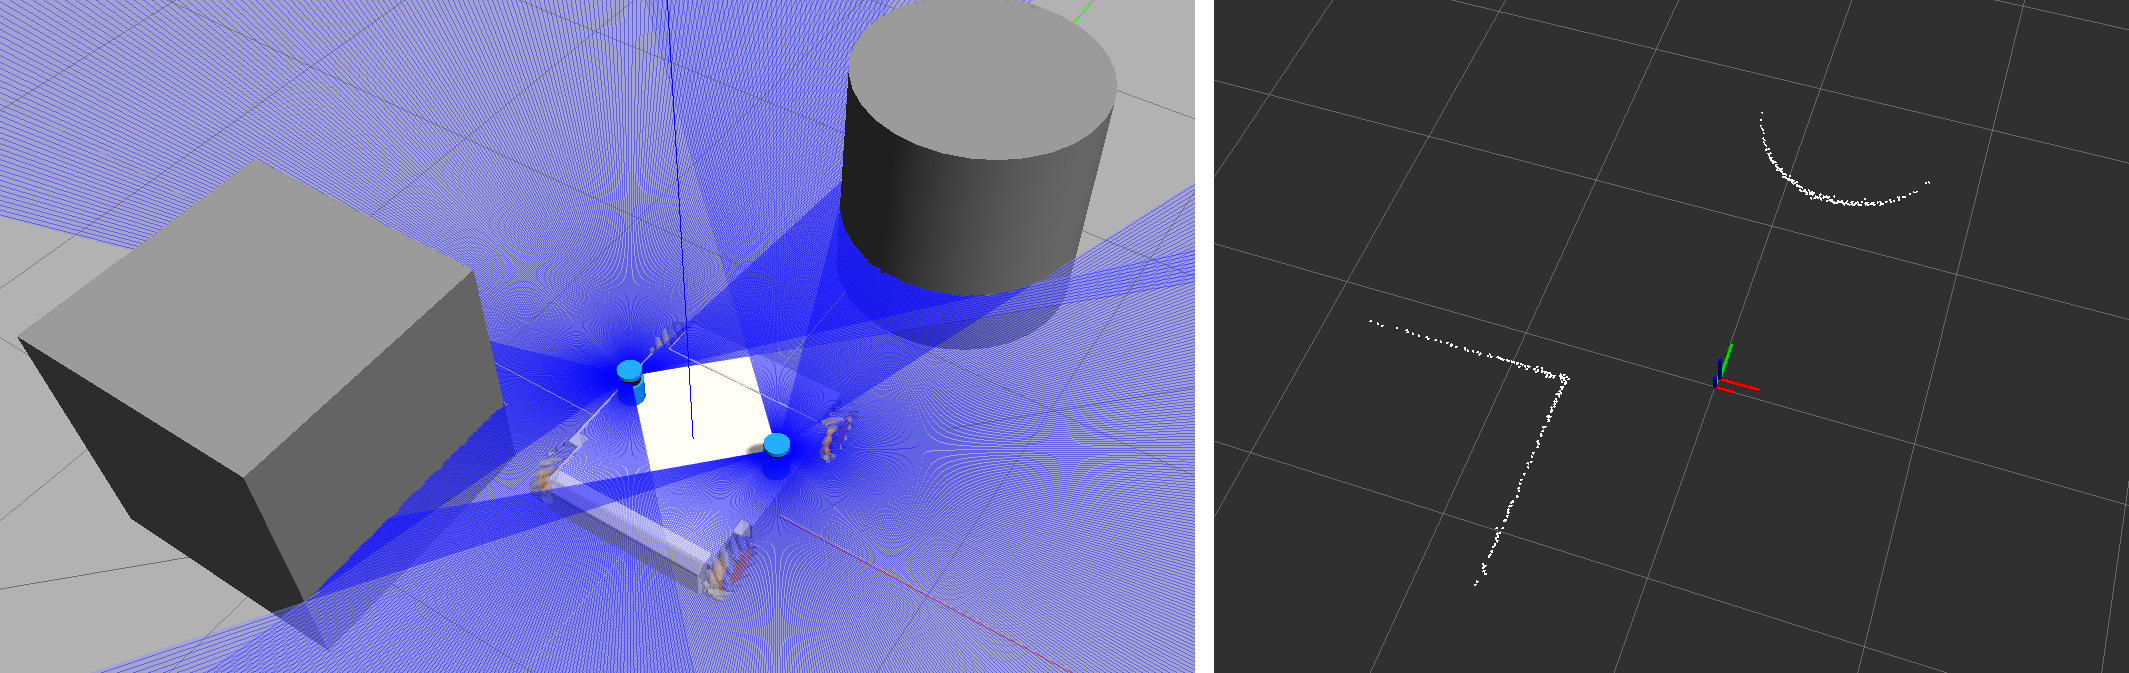
\includegraphics[width=\textwidth]{graphics/scan.png}
			\caption{Zrzut ekranu platformy z Gazebo i wygenerowane dane, obserwowane w Rviz.}
			\label{fig:scan}
			\end{figure}
			
		\subsubsection{Mechanika ramek}
			\label{sec:frames}
			Komunikacja poprzez pakiety wiadomości nie jest jedynym sposobem na przekazywanie informacji w środowisku ROS.
			Istnieje także mechanika ramek transformacji \texttt{TF2}.
			Jest to idea podobna do niezaimplementowanej funkcjonalności Gazebo, ale nie jest automatyczna i nie ogranicza się tylko do jednego programu.
			
			Ramka transformacji jest informacją o aktualnej pozycji i rotacji jakiegoś obiektu względem innego.
			Polega na wysłaniu pakietu typu \texttt{geometry\_msgs/TransformStamped} prosto do demona ROS.
			Pakiet zawiera:
			\begin{itemize}
				\item Nagłówek z czasem nadania ramki i identyfikatorem, oraz informacją względem jakiej ramki podane są poniższe dane.
				\item Nazwa nowej ramki, jaka powstanie po zastosowaniu podanej transformacji do określonej w nagłówku ramki.
				\item Lokalna pozycja.
				\item Lokalna rotacja.
			\end{itemize}
			Demon ROSa następnie zbiera wszystkie dane ze wszystkich nadających komponentów i oblicza hierarchę transformacji obiektów.
			Zwraca te dane na zapytania od innych komponentów.
			
			Przykładowo, gdyby symulacja robota nie odbywałaby się w przestrzeni wirtualnej, w maszynie symulacyjnej fizyki, 
			informacja o dokładnym położeniu obiektu składowego w lokalnym układzie współrzędnych wcale nie musiałaby być łatwo dostępna.
			Ma to szczególne znaczenie dla skomplikowanych mechanizmów, na przykład wielosegmentowego ramienia manipulacyjnego.
			Obliczenie pozycji i rotacji końcówki ramienia wymagałoby informacji o aktualnych pozycjach i rotacjach wszystkich segmentów.
			Która część systemu miałaby zajmować się obliczeniami i jaki kod powinien posiadać i gdzie przekazywać te informacje?
			
			Demon ROSa działa tutaj jak trzecia strona, zbierająca dane od przegubów i obliczająca pozycje i rotacje wszystkich punktów.
			W takim przypadku, każdy segment symulacji mógłby przekazywać swój identyfikator, identyfikator obiektu którym steruje, jego pozycję i rotację do demona ROSa.
			Inne programy, na przykład do wizualizacji, mogłyby wtedy zapytać się demona o dokładne pozycje przegubów w przestrzeni kartezjańskiej, a on obliczyłby je i zwrócił wynik.
			
			W symulacji platformy wielokierunkowej, mechanika ramek jest potrzebna, gdyż pakiet zwierający pomiary z czujnika laserowego nie posiada informacji o aktualnej
			pozycji samego czujnika w przestrzeni, a jedynie identyfikator ramki czujnika. 
			Pozycja potrzebna jest programowi obliczającemu pozycję z czujników i ewentualnemu wizualizatorowi samych danych.
			
			Symulator platformy zawiera drugi program, który w każdym cyklu symulacji nadaje demonowi ROS pozycje i rotacje środków czujników laserowych, dla uproszczenia
			względem początku układu współrzędnych, punktu (0,0,0). 
			Program sterujący modelem samej platformy także nadaje ramkę z pozycją i rotacją platformy względem globalnego środka układu współrzędnych.
			Dokładnie taki sam efekt byłby, gdyby nadawać stałą pozycję i rotację czujników laserowych, ale względem ramki platformy (nadawanej przez inny sterownik).
			Stałą, ponieważ czujniki nie zmieniają swojej pozycji na platformie, są przytwierdzone na stałe.
			
			\begin{table}
				\centering
				\begin{tabular}{l r}
					Punkt ramki & Nazwa punktu \\
					\hline
					Stały środek mapy & \texttt{map} \\
					Środek platformy & \texttt{omnivelma} \\
					Środek platformy kinematycznej & \texttt{pseudovelma} \\
					Emiter prawego lasera & \texttt{monokl\_r\_heart} \\
					Emiter lewego lasera & \texttt{monokl\_l\_heart} \\
				\end{tabular}
				\caption{Nazwy identyfikatorów ramek, używanych w symulatorze.}
				\label{tab:frames}
			\end{table}
				
			\begin{table}
				\centering
				\begin{tabular}{l c r}
					Nazwa & Punkt względny & Punkt danych \\
					\hline
					Pozycja i rotacja platformy & \texttt{map} & \texttt{omnivelma} \\
					Pozycja i rotacja platformy kinematycznej & \texttt{map} & \texttt{pseudovelma} \\
					Pozycja i rotacja prawego czujnika & \texttt{map} & \texttt{monokl\_r\_heart} \\
					Pozycja i rotacja lewego czujnika & \texttt{map} & \texttt{monokl\_l\_heart} \\
				\end{tabular}
				\caption{Ramki wysyłane do demona ROS.}
				\label{tab:frame_send}
			\end{table}

	\subsection{Błędy}
		Jak podano wcześniej w tabelce \ref{tab:lidar}, wyróżnione są dwa typy błędów pomiaru, systematyczny i pomiarowy.
		Dodatkowo istnieje także błąd gruby.
		Model czujnika powinien uwzględniać wszystkie błędy, aby zwracać dane jak najbardziej zbliżone do LiDARa.

		\subsubsection{Błąd gruby}
			Najprostszy typ błędu polega na dużych odchyłach niektórych pomiarów od pozostałych wartości.
			W trakcie przetwarzania odczytu, te punkty powinno się odrzucić.
			Nie mniej jednak, to zadanie należy do programu sterującego, więc należy umożliwić mu testowanie tej funkcjonalności poprzez wprowadzenie takich błędów do zasymulowanych odczytów.

			Najczęstszym przypadkiem błędu grubego jest brak odbioru wysłanego impulsu. 
			To skutkuje nadaniem aktualnemu pomiarowi wartości maksymalnej, co jest bardzo łatwo wykryć i usunąć.

			Innym problemem może być odebranie światła niepochodzącego od emitera urządzenia, a jakiegoś zewnętrznego źródła.

			Ponieważ rozkład i częstotliwość tych błędów zależy od środowiska w jakim działa czujnik, bardzo ciężko jest dobrać odpowiedni algorytm ich generacji.
			%TODO dopisać po implementacji

		\subsubsection{Błąd systematyczny}
			Ten błąd jest stałą wartością, dodaną do każdego pomiaru.
			Spowodowany jest niedoskonałością budowy elementów pomiarowych, niewłaściwą kalibracją, zużyciem, lub otoczeniem w jakim pracuje czujnik.

			Rzeczywisty LiDAR powinien być skalibrowany przed użyciem właśnie po to, aby wewnętrzny program sterujący mógł obliczyć aktualne zboczenia pomiarów
			i skorygować dane przed wysłaniem ich wyżej.
			Czujnik może także wysyłać czyste i obarczone błędami dane do programu sterującego, który samodzielnie je skoryguje.
			Pozwoli to na zastosowanie dowolnych algorytmów oczyszczania danych, kosztem większego obciążenia programu sterującego.

			Symulator czujnika powinien mieć interfejs do ustawienia tej wartości, aby mógł być ,,skalibrowany'' w taki sam sposób, jak faktyczne urządzenie.
			%TODO dopisać po implementacji

		\subsubsection{Błąd pomiarowy}
			Jest to mała, losowa wartość, dodana do każdego pomiaru.
			Wynika ona z niedoskonałości samego czujnika, nieznanych zakłóceń i niezbadanych efektów kwantowych.
			Nie da się w żaden sposób usunąć, zmniejszyć, lub przewidzieć tego typu błędów.
			Jedynym sposobem jest obliczenie średniej błędu na podstawie dużej ilości pomiarów.

			Błąd pomiarowy ma zwykle rozkład normalny o określonym odchyleniu standardowym.
			Standard SDF przewiduje element określający tę liczbę, a Gazebo może wewnętrznie obliczyć i dodać do wyników odpowiednią wartość.
			Również producent podał w tabeli danych urządzenia obliczony rozkład standardowy.

			W związku z tym, wartość podana przez producenta, podana w tabelce \ref{tab:lidar}, może być bezpośrednio zapisana do 
			elementu odchylenia standardowego, w pliku SDF opisującym czujnik.
			Wadą takiego rozwiązania jest niemożność modyfikacji tego parametru w trakcie wykonywania programu, gdyż Gazebo nie wystawia API do modyfikacji tej wartości.
			Aby temu zaradzić, wystarczy obliczać błąd standardowy w programie sterującym i manualnie dodawać go do zwróconej przez symulator tablicy danych.
			Funkcje do obliczania błędu standardowego zostały wprowadzone do standardu języka C++ w 2011 roku.
			
			Na zrzucie ekranu \ref{fig:scan} można zobaczyć, iż punkty pomiarów, wizualizowane w RViz, nie leżą idealnie na figurach powstałych poprzez przecięcia skanowanych brył.
			Dodany jest szum, jak gdyby rozmazujący punkty.

\section{Model czujnika inercji}
	Ponieważ czujniki tego typu są często stosowane w robotyce, wszystkie komponenty systemu wspierają jego symulację i struktury przekazywanych danych.
	\begin{itemize}
		\item ROS posiada specjalną wiadomość typu \texttt{sensor\_msgs/Imu}, do przekazywania pomiarów pomiędzy komponentami.
		\item SDF definiuje element typu \texttt{imu} w sekcji czujników, gdzie można mu zdefiniować położenie w robocie i współczynniki błędów pomiarowych.
		\item Gazebo daje wsparcie klasy czujnika inercji z odczytem wygenerowanych przez maszynę symulacji wartości.
	\end{itemize}
	
	Ten czujnik podłączony jest do platformy dynamicznej.
	
	Warto tutaj nadmienić, że struktura wiadomości ROSa posiada pola dla danych, które nie koniecznie mogą być wygenerowane przez czujnik rzeczywisty.
	Takimi polami jest struktura rotacji, zapisana jako kwaternion, oraz macierze kowariancji, wyznaczane zewnętrznie eksperymentalnie.
	
	Macierze kowariancji definiują wpływ danych z jednej osi na drugą i mnożniki wyjścia. 
	Nierówność pomiarów na przykład może być to spowodowana odchyleniem akcelerometrów względem kąta prostego, co powoduje że ruch w osi jednego czujnika może
	być także wykryty przez czujniki innych osi. 
	Podobnie jest, gdy czujniki nie generują dokładnie tych samych danych na taki sam ruch wzdłuż ich osi, co może być spowodowane niedokładnością wykonania elementów.
	Macierz pozwala zastosować te cechy sprzętowe do danych w celu poprawy ich jakości.
	
	W większości programów używających przestrzeń wirtualną, rotację zapisuje się w postaci kwaterniona, jako cztery liczby.
	Taka postać odporna jest na zjawisko utraty jednego ze stopni swobody (\emph{gimbal lock}), gdy dwie z trzech osi pokryją się, niemożliwy staje się obrót obiektu wokół trzeciej osi. Niestety, taka postać nie ma odwzorowania w rzeczywistej przestrzeni.
	
	Symulacja żyroskopu w maszynie symulacyjnej fizyki jest bardzo prosta, gdyż algorytm wyznaczania pozycji obiektów na podstawie nadanych sił korzysta wewnętrznie z
	wartości prędkości dla każdego obiektu. Zatem kwestia symulacji tego sensora polega na odczycie odpowiednich struktur w maszynie symulacji.
	Wtyczka do Gazebo, zapisana podobnie do wtyczki czujnika laserowego, zbiera w każdym cyklu maszyny symulacyjnej dane i wysyła ja za pomocą pakietu ROSa.
	
	Akcelerometr jest bardziej złożonym problemem, gdyż maszyna symulacji działa w czasie dyskretnym, co utrudnia różniczkowanie prędkości w celu otrzymania przyspieszenia.
	Ta wartość nie jest także nigdzie indziej używana i musi być obliczona specjalnie dla symulacji tego czujnika.
	Fakt, że małe odchylenia w zmianie prędkości powodują duże skoki danych przyspieszenia, wprowadza naturalny szum do generowanych danych.
	W sekcji \ref{sec:test_imu}, sekcji testów, opisane zostały te problemy dokładniej.
	
	Pomimo, że odczytanie tych wartości jest tak samo proste, jak prędkości kątowej, to generowane dane różnią się jakością.
	Szum jest większy, a co za tym idzie, potrzeba dodatkowego programu do odszumienia wygenerowanych wartości.
	Ten komponent jest opisany w sekcji \ref{sec:odszumiacz}.


\section{Manualne sterowanie}
\label{sec:lalkarz}
	To zaawansowany program do manualnego generowania zadanych prędkości, lub kierunku platformy.
	Ponieważ jest niezależny od reszty systemu, może być użyty do sterowania rzeczywistym robotem.
	Pozwala także na wyświetlanie aktualnych prędkości kół, generowanych przez enkodery.
	Ma nazwę kodową \texttt{lalkarz}, ponieważ steruje platformą, tak jak aktor steruje marionetką.
	
	\subsection{Program}
		Ten komponent jest plikiem wykonywalnym, skompilowanym ze źródeł w C++.
		Wykorzystując bibliotekę graficzną SFML, generuje okno z powierzchnią do rysowania na nim za pomocą OpenGL.
		Biblioteka ta pozwala również na bezproblemowe przechwytywanie zdarzeń z klawiatury, takich jak wciśnięcie i puszczenie klawisza, a także na obsługę kontrolera go gier i myszki.
		Za pomocą gałek kontrolera, można nadawać robotowi niebinarne prędkości kół, co jest niezbędne do płynnego i bezpiecznego kontrolowania urządzeniem.
		Użyto także sterowania kursorem myszy, w razie gdyby użytkownik nie posiadał kontrolera.
		
		Aplikacja tego typu mogłaby bez większego problemu pracować z interfejsem tekstowym w terminalu, aby być bardziej przenośna i lżejsza w zasobach, 
		lecz nie mogłaby wykrywać zdarzeń puszczenia klawisza
		(bez bezpośredniego czytania z urządzenia \texttt{/dev/input/eventX}, do czego są potrzebne prawa roota). 
		Dodatkowo, interfejs graficzny pozwala na wyświetlenie dokładniejszych wskaźników i elementów wskazujących.
		
		Program uruchamiany jest z wiersza polecenia, z argumentami dotyczącymi nazw strumieni i początkowej konfiguracji urządzenia.
	
	\subsection{Komunikacja}
		Program potrafi generować dwa typy wiadomości.
		
		Pierwszą są prędkości kół \texttt{omnivelma\_msgs/Vels}, jakie w danej chwili platforma powinna przyjąć na sterowanie.
		Pozwala to na dokładne przetestowanie zachowania się modelu platformy.
		Można także wywołać takie prędkości, które nie powinny być używane przy rzeczywistym sterowaniu, gdyż wprowadzają duże nieścisłości ruchu 
		(przykładowo, obracanie przednich i tylnych kół tak, aby ich wektory prędkości się znosiły, będzie nadawać niedeterministyczny ruch, spowodowany niedoskonałościami
		pojedynczych rolek).
		
		Drugi typ wiadomości, \texttt{geometry\_msgs/Twist}, to nadana prędkość względna platformy.
		To intuicyjny sposób, w jaki użytkownik steruje platformą i w jaki sposób mógłby także sterować nią prosty program sterujący.
		Jednak ponieważ ani model platformy, ani rzeczywisty robot nie są wstanie poruszać się bez informacji, jakimi kołami z jaką prędkością obracać,
		ten typ wiadomości musi być jeszcze konwertowany przez komponent modelu kinematyki odwrotnej, opisany w sekcji \ref{sec:transmutator}.
		
		Program opcjonalnie przyjmuje także wiadomość \texttt{omnivelma\_msgs/Vels}, aby wyświetlić dane enkoderów.
		Należy zauważyć, że nie przyjmuje całego pakietu \texttt{omnivelma\_msgs/EncodersStamped}, jaki jest generowany przez model platformy,
		a jedynie mały ich wycinek, gdyż tylko te informacje jest w stanie wyświetlić i tylko takie potrzebuje.
		Dzięki temu może być użyty niezależnie od innych komponentów i programów. Jednak może być wymagane użycie dodatkowego komponentu do 
		wyłuskania tej informacji z większego pakietu,
		patrz \ref{sec:dziadzio}.
		
	\subsection{Tryby działania}
		Program posiada 11 trybów działania, w których generuje różne wiadomości w różny sposób.
		Jedne są bardziej przydatne, inne bardzo proste i służące do ogólnej prezentacji systemu.
		Globalny mnożnik wyjścia pozwala na łatwe ograniczenie generowanych danych i ustawienia dokładności. Spacja awaryjnie zeruje wszystkie wyjścia.
		\begin{enumerate}
			\item Za pomocą ośmiu klawiszy klawiatury numerycznej, można nadać platformie określone prędkości kół.
			W tym trybie, koło może albo stać w miejscu, albo obracać się z odpowiednią prędkością, w określonym kierunku. 
			Powoduje to naturalne szarpnięcia i poślizgi platformy. W trakcie braku aktywności użytkownika, platforma stoi w miejscu.
			\item Podobnie do poprzedniego trybu, lecz przy braku naciśnięcia klawisza, generuje cichą nie-liczbę, aby zachować aktualną prędkość kół modelu.
			Ta dodatkowa funkcjonalność opisana jest szerzej w sekcji \ref{sec:model_nan}.
			\item Naciśnięcie klawisza płynnie zwiększa, lub zmniejsza prędkość koła. W trakcie braku aktywności użytkownika, platforma porusza się 
			z ustawionymi prędkościami kół.
			\item Podobnie, co w poprzednim trybie, lecz pozwala na schodkowe ustawienie prędkości kół co 0,1 $\frac{rad}{s}$ (pomnożone przez dokładność).
			Dzięki temu, możliwe jest w miarę dokładne powtórzenie manualnych testów platformy.
			\item Poprzedni tryb, lecz przy ustawieniu prędkości zerowej, generuje nie-liczbę.
			\item Sterowanie prędkościami kół za pomocą gałek kontrolera.
			Większość kontrolerów posiada dwa, dwuosiowe joysticki, co daje cztery osie, zmieniające się w zakresie $\left<-1;1\right>$.
			Można za ich pomocą bezpośrednio ustawiać prędkości kół, chociaż jest to nieintuicyjne w działaniu.
			\item Lokalny kierunek jazdy platformy składa się z dwóch wektorów prędkości liniowej i wektora obrotu. 
			Za pomocą klawiatury, binarnie, można nadać platformie jeden z ośmiu kierunków poruszania się i jeden z dwóch kierunków obrotu.
			Ponownie, ta metoda sterowania powoduje skoki prędkości i poślizgi. Przypomina sterowanie pojazdami w grach komputerowych.
			Puszczenie klawiszy powoduje zatrzymanie się platformy.
			\item Podobny tryb do poprzedniego, ale naciśnięcie klawisza płynnie dodaje wartość do kierunku poruszania się i obrotu platformy.
			Brak aktywności użytkownika powoduje, że model porusza się z zadaną prędkością w zadanym kierunku i z zadanym obrotem.
			\item Połączenie dwóch poprzednich trybów, schodkowe sterowanie prędkością platformy. Pozwala na ustawienie prędkości i obrotu platformy z zadaną dokładnością.
			\item Sterowanie kierunkiem platformy za pomocą kontrolera. Trzy osie są używane, dwie do nadania prędkości, jedna do nadania obrotu.
			Jest to prawdopodobnie najczęstszy sposób kontrolowania robotów wielokierunkowych za pomocą kontrolera.
			Bardzo intuicyjny i używany także przez inne pakiety do manualnego sterowania robotami na kołach Mecanum.
			\item Sterowanie za pomocą myszki, najdokładniejsze sterowanie kierunkiem, mniej dokładne obrotem.
			Kursor myszy wskazuje końcówkę strzałki reprezentującej kierunek ruchu robota, za pomocą kółka, można dodawać, lub odejmować prędkość do obrotu wokół osi.
			Ponieważ większość myszek ma skokowe obroty kółek, wprowadza to nieznaczne poślizgi. Można także modyfikować obrót klawiaturą w płynnym trybie przyrostowym.
		\end{enumerate}
		
		\begin{figure}[H]
		\centering
		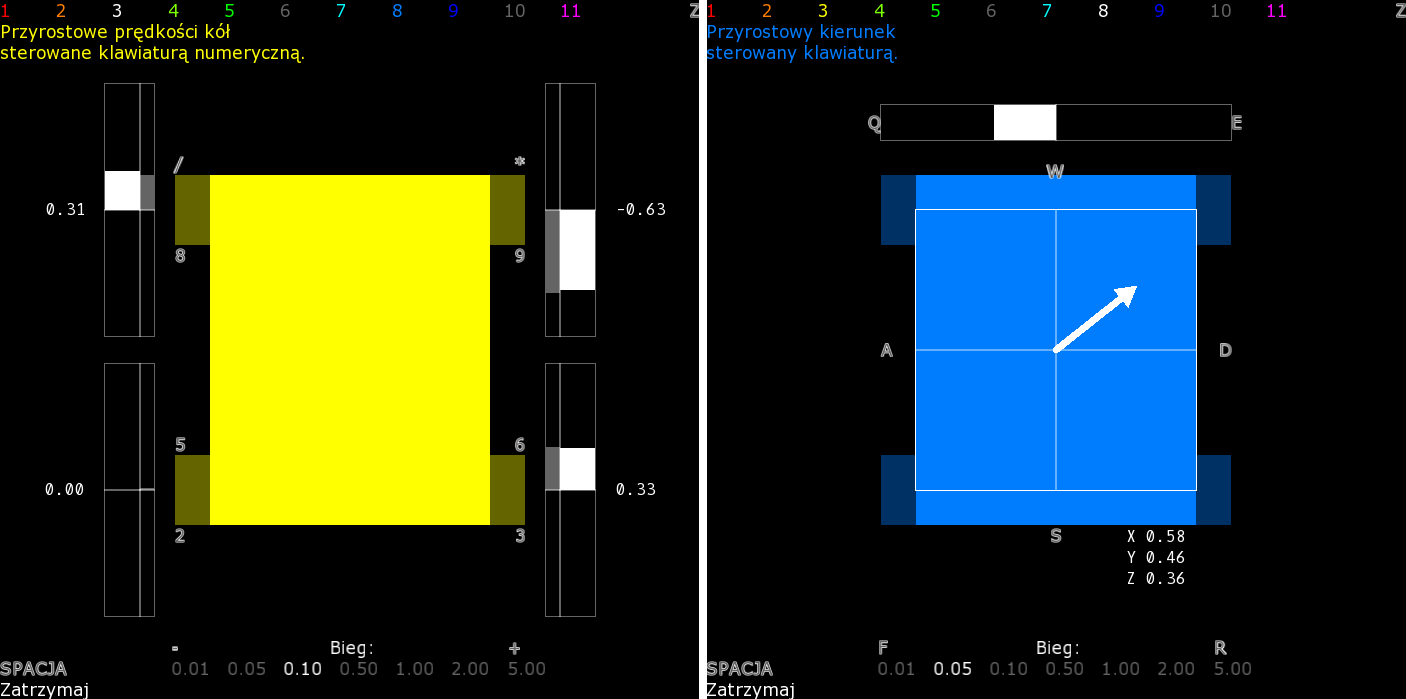
\includegraphics[width=\textwidth]{graphics/lalkarz.png}
		\caption{Zrzuty ekranu dwóch trybów działania programu.}
		\label{fig:lalkarz}
		\end{figure}
		
		Interfejs składa się z listy trybów, wyświetlanych na górze, i nazwy aktualnego trybu.
		Wyszarzone tryby nie mogą być aktywowane, w tym przypadku z powodu braku podłączenia kontrolera.
		
		Na lewym zrzucie widać zarys platformy i białe wskaźniki aktualnych prędkości kół, wraz ze współczynnikiem wypełnienia.
		Obok nich znajdują się szare wskaźniki prędkości, zwrócone przez modele enkoderów.
		Małe, szare znaki to nazwy klawiszy, używanych w tym trybie do modyfikowania prędkości.
		
		Na prawym obrazku jest tryb generowania kierunku i obrotu. Strzałka wskazuje wektor prędkości, a górny pasek obrót platformy.
		
		Na dole jest lista ,,biegów'' urządzenia, są to zwyczajne mnożniki wyjścia w celu wygodnego przestawiania dokładności z jaką platforma powinna się poruszać.
		
		Wszystkie dane są w jednostkach SI, tzn, efektywna prędkość koła będzie się równać liczbie podanej przy kole, pomnożonej przez aktualny bieg.
		Dla obrotów to są $\frac{rad}{s}$, dla prędkości to $\frac{m}{s}$.
		
\section{Generator sterowania}
	\label{sec:gramofon}
	Podstawą przeprowadzania testów modelu jest powtarzalność eksperymentów, oraz dokładność.
	Potrzeba zatem jest sposobu na automatyczne wygenerowanie strumienia wiadomości z określonymi danymi.
	
	Program \texttt{gramofon} wczytuje plik danych, w którym znajdują się rekordy, każdy opisuje:
	\begin{itemize}
		\item Prędkość liniową platformy w osi X.
		\item Prędkość liniową platformy w osi Y.
		\item Prędkość kątową platformy w osi Z.
		\item Czas $t$, przez który program ma generować wiadomość z podanymi wyżej danymi.
	\end{itemize}
	Program czyta także z argumentu okres $T$ odświeżania wiadomości.
	
	Korzystając z dwóch liczników systemowych, program generuje co $T$ sekund wiadomość typu \texttt{geometry\_msgs/Twist} z danymi aktualnie wykonywanej linii pliku.
	Ta wiadomość powtarza się regularnie.
	
	Po upływie czasu $t$, program nadaje dodatkową wiadomość z nowymi danymi, oraz przestawia dane generowane przez wywołania pierwszego licznika.
	
	Po wykorzystaniu danych, algorytm nadal generuje wiadomości z zerowymi prędkościami, aby zatrzymać model platformy i podtrzymać aktywne hamowanie kół.
	
	W ten sposób, możliwe jest proste generowanie sterowania robota, bazujące na czasie.
	Przykładowo, program może generować sterowanie:
	\begin{enumerate}
		\item Ruch przez 3,2 s, z prędkością 0,2 $\frac{m}{s}$, w kierunku (2,1).
		\item Zatrzymanie na czas 0,9 s.
		\item Obrót przez czas 10 s, z prędkością kątową 0,02 $\frac{rad}{s}$.
	\end{enumerate}
	
	Ponieważ jednak system operacyjny, na którym pracuje program i symulator, nie spełnia wymogów systemu czasu rzeczywistego, generowane wiadomości
	nie muszą być (i nie są) wysyłane dokładnie w określonych momentach. Można przeprowadzić prosty eksperyment, aby zaprezentować ten problem.
	
	\begin{figure}[H]
	\centering
	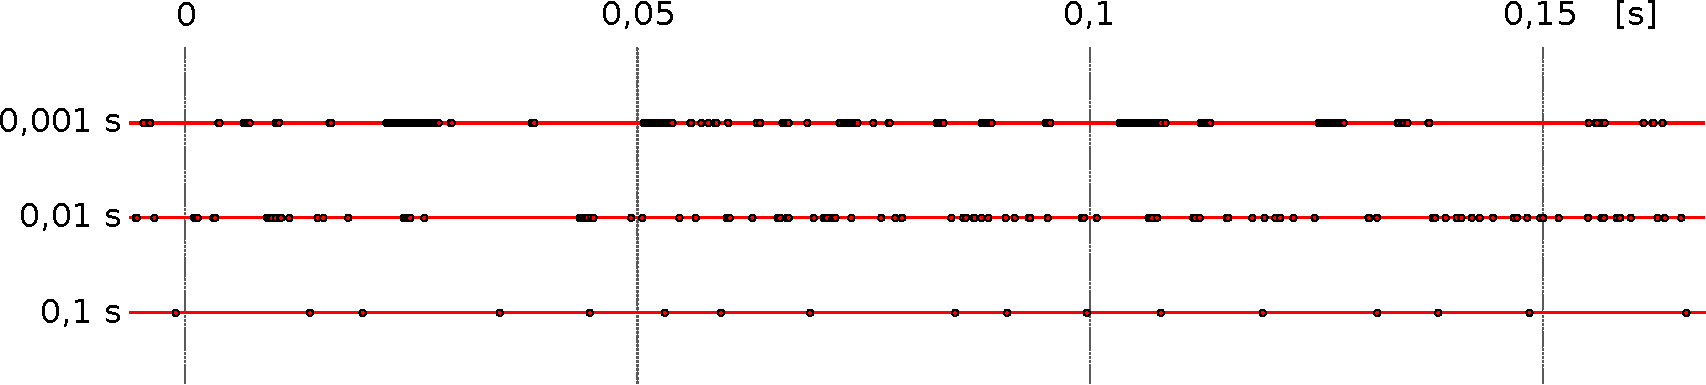
\includegraphics[width=\textwidth]{graphics/gramofon.pdf}
	\caption{Czas odbioru pakietu, wysyłanego przez program działający z jednym z trzech okresów.}
	\end{figure}
	
	Działa to tak samo, jakby każdą wiadomość wysyłać z losowym opóźnieniem.
	Gdy nadań jest za dużo (górny wykres), system zaczyna je buforować, a co za tym idzie, nadaje je w grupach o losowej wielkości.
	Pakiet po nadaniu przechodzi przez wiele procesów, każdy może nadawać losowe opóźnienie dla wiadomości.
	System operacyjny pod dużym obciążeniem przez inne procesy będzie opóźniał i buforował wiadomości o niższych częstotliwościach.
	
	Aby rozwiązać ten problem, należałoby uruchomić całe środowisko ROSa na systemie operacyjnym czasu rzeczywistego.
	Jedynym takim systemem, eksperymentalnie wspieranym przez twórców ROSa, jest OpenEmbedded.
	Jednakże budowa i uruchomienie tego systemu jest bardzo złożone.
		
\section{Wyłuskanie struktury wiadomości}
	\label{sec:dziadzio}
	Każda wiadomość przekazywana pomiędzy komponentami jest zwykle zagnieżdżoną strukturą.
	Na przykład pakiet typu \texttt{geometry\_msgs/Twist} składa się z dwóch podstruktur wektorów trójwymiarowych.
	Jeden odpowiada za prędkość, a drugi za rotację.
	
	Czasami może zdarzyć się, że jakiś komponent potrzebuje jedynie wewnętrznej podstruktury pakietu.
	Nie powinno mu się zatem przekazywać całej struktury wiadomości, gdyż to powodowałoby niepotrzebne opóźnienia, oraz nie pozwoliłoby zachować niezależności 
	komponentu od innych.
	
	Takie zjawisko występuje przy przekazywaniu informacji o pozycji i prędkości kół, generowanej przez model czujnika enkoderów, do programu
	manualnego sterowania, opisanego w \ref{sec:lalkarz}.
	
	ROS nie pozwala na automatyczne odbieranie tylko części pakietu, dlatego powstał program o nazwie kodowej \texttt{dziadzio}, niczym dziadek do orzechów.
	Przyjmuje wiadomości typu \texttt{omnivelma\_msgs/EncodersStamped} i zwraca wiadomości typu \texttt{omnivelma\_msgs/Vels}, który to typ 
	jest zawarty wewnątrz przyjmowanej struktury. Pozwala to na połączenie modelu czujnika enkoderów z wyświetlaczem prędkości kół w programie do manualnego sterowania.

\section{Podłoga o zmiennym współczynniku tarcia}
	\label{sec:flooria}
	Symulacja nie składa się jedynie z robota i czujnika, ale także z podłoża, na którym musi się poruszać.
	Ponieważ podłoże również wpływa na symulację, powinien istnieć sposób na ustawienie jego współczynnika tarcia.
	Robi się to wewnętrznie w identyczny sposób, jak w przypadku kół platformy, co zostało opisane w sekcji \ref{sec:friction}.
	
	W tym przypadku jednak powinno się ustawić identyczne wektory tarć $F_1$ i $F_2$, aby podłoże symulowało równe tarcie we wszystkich kierunkach.
	Tak samo, jak w przypadku modelu platformy dynamicznej, program nadający podłożu odpowiednie wektory tarcia przyjmuje asynchroniczne wywołanie 
	typu \texttt{omnivelma\_msgs/SetFriction}, zawierające dwie wartości zmiennoprzecinkowe.
	
	Nazwa kodowa tego programu sterującego to \texttt{flooria}, od angielskiej nazwy na podłogę.
	Program jest uruchamiany jako biblioteka symulatora Gazebo.
	
\section{Algorytm usuwania szumu z danych modelu czujnika inercji}
	\label{sec:odszumiacz}
	Jak wcześniej wspomniano, różniczkowanie prędkości w maszynie symulacji fizyki generuje duże błędy.
	
	Ten program uśrednia dane w prosty sposób, licząc średnią z określonej ilości poprzednich pomiarów.
	Odczytuje nazwę nadajnika i odbiornika wiadomości typu \texttt{sensor\_msgs/Imu}, oraz wielkość bufora,
	
	Taki algorytm nie sprawdza się jednak, gdy dane są generowane naprzemiennie.
	Na przykład, jeśli w jednej klatce symulacji maszyna do symulacji fizyki obliczy prawidłową wartość, a w drugiej zwróci zerową,
	to ten algorytm uśredni te wyniki i zwróci wartość pośrodku.
	
	Jednak stworzenie tego komponentu pozwoliło sprawdzić, czy model czujnika inercji reaguje na ruch platformy z określonymi przyspieszeniami.
	Pozwolił także na odkrycie innych cech generatora.
	Używany jest w przeprowadzeniu testów w sekcji \ref{sec:test_imu}. Nazwa kodowa to \texttt{odszumiacz}.
	
\section{Obserwator symulacji}
	\label{sec:ocznica}
	Kolejny program uruchamiany w symulatorze Gazebo, oblicza i zwraca ciąg danych, reprezentujący 
	odległość i kąt pomiędzy platformą dynamiczną i kinematyczną, pakiet \texttt{omnivelma\_msgs/Relative}.
	Te dane pozwalają sprawdzić, na ile symulacja fizyczna opóźnia się względem matematycznego modelu.
	
	Ten program nie może być zaimplementowany jako zewnętrzny komponent, gdyż wiadomości zawierające pozycje platform będą przychodzić asynchronicznie.
	Nie da się w takim przypadku obliczyć dokładnych odległości pomiędzy platformami w danej chwili. 
	Wprowadzałoby to także spore opóźnienie, gdyż program musiałby czekać na odbiór obu pakietów, dodatkowo zachowując pewność że oba pochodzą z tej samej klatki symulacji.
	
	Nazwa kodowa tego programu to \texttt{ocznica}.
	
\section{Model kinematyki odwrotnej}
	\label{sec:transmutator}
	Jest to model kinematyki odwrotnej, alternatywa do modelu kinematycznego, opisanego w sekcji \ref{sec:pseudovelma}, jednak działającego bez symulatora i bez możliwości 
	całkowania prędkości (i generowania danych o aktualnej pozycji).
	Ten komponent przyjmuje zadaną prędkość, kierunek i obrót platformy, a zwraca prędkości kół, które powinny być nadane platformie, aby wywołać taki ruch.
	
	\begin{equation}
	\begin{bmatrix}
	\omega_1 \\
	\omega_2 \\
	\omega_3 \\
	\omega_4 \\
	\end{bmatrix}
	=
	\frac{1}{r}
	\begin{bmatrix}
	1 & -1 & \frac{a+b}{2} \\
	1 & 1 & -\frac{a+b}{2} \\
	1 & -1 & -\frac{a+b}{2} \\
	1 & 1 & \frac{a+b}{2} \\
	\end{bmatrix}
	\begin{bmatrix}
	v_y \\
	v_x \\
	\omega_z \\
	\end{bmatrix}
	\end{equation}
	
	Stałe, użyte we wzorze zdefiniowane są w tabeli \ref{tab:dims}, a numerowanie kół na rysunku \ref{fig:base_dims}.
	Ten wzór, podobnie jak poprzedni, pojawia się w wielu pracach, na przykład \cite{wheels}, dokładny wygląd macierzy zależy od numerowania kół i interpretacji kierunków osi.
	
	Dodatkowo, program pozwala na obrót wektora prędkości o kąt prosty, lub półpełny. 
	Jest to spowodowane tym, że różne komponenty i różne modele przyjmują różną pozycję wyjściową robota.
	Czasami przód modelu skierowany jest w dodatnią stronę osi X, a czasami Y. W związku z tym, ta funkcjonalność jest w stanie przekonwertować dane wejściowe dla innego robota.
	
	Nazwa kodowa to \texttt{transmutator}, wykonuje transmutację jednego typu prędkości w inny.
	
\section{Mapa z symulacją}
	Symulator Gazebo przy uruchomieniu ładuje plik zawierający referencje robotów i ich początkowe pozycje, używane w symulacji.
	Ten pakiet nie jest programem wykonywalnym, lecz prezentuje informacje dla symulatora o scenie symulacji.
	
	Plik typu \texttt{world} jest plikiem SDF, podobnym do tych, które służą do określenia wewnętrznej budowy robotów.
	Posiada listę elementów \texttt{import} ze ścieżkami modeli, a także nazwy programów działających bez modelu, jak obserwator symulacji, opisany w sekcji \ref{sec:ocznica}.

	W tym pliku zawierają się także ustawienia symulacji, jak przyspieszenie grawitacyjne, typ maszyny symulacyjnej fizyki ze współczynnikami, czy ustawienia wirtualnej atmosfery.
	
	Nazwa komponentu \texttt{velmaverse} jest zlepkiem słów ,,universe'' i nazwy robota manipulacyjnego.
	
\section{Rozdzielacz pakietów}
	Jeśli dwóm komponentom nadać te same nazwy interfejsów, to ROS będzie przekazywał pomiędzy nimi informacje.
	To jednak nie zawsze jest możliwe, aby mieć całkowitą kontrolę nad nazwami interfejsów wszystkich komponentów.
	Dlatego też, potrzeby jest program do przekazywania i ewentualnego rozdzielania pakietów dla różnych odbiorników.
	
	Ten program wykonywalny pobiera i generuje wiadomości typu \texttt{omnivelma\_msgs/Vels}, zawierające prędkości kół.
	Pozwala to na sterowanie kilkoma robotami o identycznym interfejsie ze wspólnego źródła.
	W szczególności przydaje się to przy rozdzielaniu wartości prędkości kół dla modelu platformy dynamicznej i kinematycznej.
	
	Nazwa kodowa \texttt{widelnica} jest referencją do widelca którego końcówka rozdziela się na kilka części, a także do angielskiej nazwy ,,fork'', używanej w podobnych 
	przypadkach rozdzielania informacji.
	
\section{Prosty program sterujący}
	Jest to uproszczona wersja programu, który docelowo ma być tworzony na podstawie budowanego systemu modeli.
	Pozwala on sprawdzić, jak dla prostych zasad model będzie się zachowywał.
	
	Program periodycznie wysyła wiadomość typu \texttt{geometry\_msgs/Twist} o kierunku równoległym do osi współrzędnych.
	W zależności od danych z czujników laserowych, program zmienia swój stan i obraca kierunek obrotu o 90\textdegree.
	Ten sterownik dla uproszczenia nie generuje poleceń obrotu kątowego, model powinien być zawsze zwrócony w tę samą stronę.
	
	Działanie programu oparte jest na zachowaniu akcja-reakcja.
	Dane z czujników laserowych dzielone są, w zależności od kąta pomiaru, na cztery ćwiartki lokalnego układu współrzędnych.
	Rozpatrywane są tylko te ćwiartki, w których kierunku porusza się platforma.
	Jeśli pomiar wypadnie wystarczająco blisko platformy, kierunek jest obracany w odwrotnym do tej ćwiartki kierunku.
	
	Na przykład, jeśli platforma porusza się w prawo i wykryje obiekt w trzeciej ćwiartce (czyli po prawej stronie względem aktualnego kierunku poruszania się),
	to zacznie poruszać się prosto, aby uniknąć przeszkody.
	
	Taki program gwarantuje omijanie przeszkód, aby platforma nie zderzyła się z jakimś obiektem.
	
	Nazwa kodowa \texttt{pantofelek} pochodzi z tego, że zachowuje się jak taki pierwotniak.
	
\section{Struktury pakietów wiadomości}
	Ten komponent nie jest plikiem wykonywalnym, a definicjami struktur danych, używanych przez wiadomości ROSa w projekcie, jeśli 
	standard nie obejmuje potrzebnego typu wiadomości.
	Nazwa kodowa i jednocześnie przedrostek wszystkich zawartych typów to \texttt{omnivelma\_msgs}.

\section{Zewnętrzne pakiety}
	Istnieje kilka tysięcy różnych pakietów i programów, tworzonych przez społeczność ROSa.
	
	\subsection{Rysownik wykresów}
		Pakiet \texttt{rqt-multiplot} jest wtyczką do większego programu \texttt{rqt}.
		Pozwala na generowanie dwuwymiarowych wykresów, bazując na dwóch dowolnych wartościach z odbieranych pakietów, lub czasie.
		Można porównać różne wykresy na jednym układzie.
		
		W szczególności przy ustawieniach pozycji Y względem X, pobranych z pakietu pozycji, nadawanego przez obie platformy, pozwala narysować trajektorię ruchu platform.
	\subsection{Wizualizer pomiarów}
		Oryginalnie napisany dla robota o tej samej nazwie, \texttt{rviz} prezentuje trójwymiarową przestrzeń, na której można wyświetlać 
		dane odebrane z pakietów.
		
		Pozwala to na przykład umieścić znacznik platformy i chmury punktów odebranych z czujników laserowych.
		Jest lżejszy na zasobach w działaniu niż Gazebo i pokazuje tylko informacje z odebranych danych, a nie całe środowisko symulacji.
		
	\subsection{Zbieranie danych}
		Każdy \texttt{topic} może zostać zapisany do pliku, a następnie odtworzony w ten sam sposób.
		Wbudowane w ROSa narzędzie \texttt{rosbag} pozwala ,,nagrać'' i odtworzyć dane dokładnie w taki sam sposób, w jaki zostały odebrane.
		Zapisuje to w formie pliku binarnego, wraz z dokładnymi parametrami działania nadajnika wiadomości.
		Możliwe jest również wydrukowanie danych do pliku tekstowego, aby mógł być wykorzystany przez inne programy jak Gnuplot, Calc (Exel), czy Matlab.
		
	
	
	
	
	

